\documentclass[10pt]{report}
\usepackage[utf8]{inputenc}
\usepackage[italian]{babel}
\usepackage{multicol}
\usepackage[bookmarks]{hyperref}
\usepackage[a4paper, total={18cm, 25cm}]{geometry}
\usepackage{graphicx}
\usepackage{xcolor}
\usepackage{textcomp}
\graphicspath{ {./img/} }
\usepackage{listings}
\usepackage{makecell}

\definecolor{backcolour}{RGB}{255,255,255}
\definecolor{codegreen}{RGB}{27,168,11}
\definecolor{codeblue}{RGB}{35,35,205}
\definecolor{codegray}{RGB}{128,128,128}
\definecolor{codepurple}{RGB}{205,35,56}
\lstdefinestyle{myPython}{
	backgroundcolor=\color{backcolour},   
	commentstyle=\color{codegreen},
	keywordstyle=\color{codeblue},
	numberstyle=\tiny\color{codegray},
	stringstyle=\color{codepurple},
	basicstyle=\small\ttfamily,
	breakatwhitespace=false,         
	breaklines=true,                 
	captionpos=b,                    
	keepspaces=true,                 
	numbers=left,                    
	numbersep=2pt,                  
	showspaces=false,                
	showstringspaces=false,
	showtabs=false,                  
	tabsize=2,
	language=python
}
\begin{document}
\title{Computational Mathematics for Learning and Data Analysis}
\author{Federico Matteoni}
\date{A.A. 2021/22}
\renewcommand*\contentsname{Index}

\maketitle
\begin{multicols}{2}
\tableofcontents
\end{multicols}
\pagebreak
\section{Introduction}
Exam: project (groups of 2) + oral exam.\\
This course's goals is to make sense of the huge amounts of data, take something big and unwieldy and produce something small that can be used, a \textbf{mathematical model}.\\
The mathematical model should be accurate, computationally inexpensive and general, but generally is not possible to have all three. General models are convenient (work once, apply many), they are parametric so we need to learn the right values of the parameters. Fitting is finding the model that better represents the phenomenon given a family of possible models (usually, infinitely many). Is an optimization model and usually is the computational bottleneck.\\
ML is better than fitting because fitting reduces the training error, the empirical risk, but ML reduces the test error, so the generalization error.\\
Solve general problem $min_{x\in S}f(x)$, with Poloni solve $min_{x\in R^n}||Ax - b||_2$ which is easier and can be solved exactly.
\chapter{Numerical Analysis}
\section{Quick recap of linear algebra}
\begin{list}{}{}
	\item \textbf{Matrix - Vector multiplication}, with $A\in R^{4\times 3}, c\in R^3, b\in R^4$
	$$\left[\begin{array}{c c c}
		A_{11} & A_{12} & A_{13}\\
		\vdots & \vdots & \vdots\\
		A_{41} & A_{42} & A_{43}
	\end{array}\right]\cdot \left[\begin{array}{c}
		c_1\\c_2\\c_3
	\end{array}\right] = \left[\begin{array}{c}
		b_1\\b_2\\b_3\\b_4
	\end{array}\right]\:\:\:\:\:\:\begin{array}{l}
		b_i = \sum_{j=1}^4 A_{ij}c_j\\
		A_{11}c_1 + A_{12}c_2 + A_{13}c_3 = b_1
	\end{array}$$
	or linear combination of the columns
	$$\left[\begin{array}{c}
	A_{11}\\A_{21}\\A_{31}\\A_{41}
	\end{array}\right]c_1 + \left[\begin{array}{c}
	A_{12}\\A_{22}\\A_{32}\\A_{42}
	\end{array}\right]c_2 + \left[\begin{array}{c}
	A_{13}\\A_{23}\\A_{33}\\A_{43}
	\end{array}\right]c_3 + \left[\begin{array}{c}
	A_{14}\\A_{24}\\A_{34}\\A_{44}
	\end{array}\right]c_4 = \left[\begin{array}{c}
	b_1\\b_2\\b_3\\b_4
	\end{array}\right]$$
	with $c_1, c_2, c_3$ and $c_4$ called coordinates.
	\item \textbf{Basis}: tuple of vectors $v_1, v_2, \ldots, v_n\:|\:$ you can write all vectors $b$ in a certain space as a linear combination $v_1\alpha_1 + v_2\alpha_2 + \ldots + v_n\alpha_n$ with \textbf{unique} $a_1,\ldots,a_n$. The canonical basis is 
	$$c_1 = \left[\begin{array}{c}
	1\\0\\0\\0
	\end{array}\right]\:\:\:c_2 = \left[\begin{array}{c}
	0\\1\\0\\0
	\end{array}\right]\:\:\:c_3 = \left[\begin{array}{c}
	0\\0\\1\\0
	\end{array}\right]\:\:\:c_4 = \left[\begin{array}{c}
	0\\0\\0\\1
	\end{array}\right]$$
	and, for example $$\left[\begin{array}{c}
	3\\5\\7\\9
	\end{array}\right] = \left[\begin{array}{c}
	1\\0\\0\\0
	\end{array}\right]\cdot 3 + \left[\begin{array}{c}
	0\\1\\0\\0
	\end{array}\right]\cdot 5 + \left[\begin{array}{c}
	0\\0\\1\\0
	\end{array}\right]\cdot 7 + \left[\begin{array}{c}
	0\\0\\0\\1
	\end{array}\right]\cdot 9$$
	\item \textbf{Image} $Im A$ = set of vectors $b$ that we can reach with $A$
	\item \textbf{Kernel} $Ker A$ = set of vectors $x\:|\: Ax = 0$ ($x = 0$ is certainly one, there may be others)
	\item \textbf{Invertible} $A$ if this problem has exactly one solution.\\
	$\forall\:b\in R^m$, $A$ must be square and the columns of $A$ are a basis of $R^m \Rightarrow x=A^{-1}b$ where $A^{-1}$ is another square matrix$\:|\: A\cdot A^{-1} = A^{-1}\cdot A = I$ identity matrix (1 on the diagonal, 0 otherwise)\\
	Implementation detail: \texttt{inv(A) * b} is not the best choice. Better: in Python \texttt{scipy.linalg.solv(A, b)} or, in Matlab, \texttt{A \ b}.
	\item \textbf{Cost}, with $A\in R^{m\times n}, B\in R^{n\times p}, C\in R^{m\times p}$ (vectors $\Leftrightarrow n\times 1$ matrices), then the cost of multiplication is $mp(2n-1)$ floating point ops (\textit{flops}), or $O(mnp)$.\\
	In particular, $A, B$ squared $\Rightarrow AB$ costs $O(m^3)$. With $A, v$ vector $\Rightarrow$ $Av$ costs $O(m^2)$. Faster alternatives are not worth it usually. And remember that $AB \neq BA$ generally, and also that $CA = CB \not\Rightarrow A = B$ with $C$ matrix.\\
	If there's $M\:|\: MC = I$, then $A = (MC)A = (MC)B = B$ (multiplying \textit{on the left} by $M$ on both sides)
\end{list}
\paragraph{} Why a real valued function? Strong assumption, given $x'$ and $x''$, I can always tell which one I like best (\textbf{total order} of R). Often more than one objective function, with contrasting and/or incomparable units (ex: loss function vs regularity in ML).\\
But $R^k$ with $k > 1$ has no total order $\Rightarrow$ no \textit{best} solution, only non-dominated ones.\\
Two practical solutions: maximize return with budget on maximum risk or maximize...\\
Even with a single objective function optimization is hard, impossible if $f$ has no minimum in $X$ (so, the problem $P$ is unbounded below. Hardly ever happens in ML, because loss and regularization are $\geq 0$\\
Also impossible if $f > -\infty$ but $\not\exists x$, for example in $f(x) = e^x$. However plenty of $\epsilon$-approximate solutions ($\epsilon$-optima). On PC $x\in R$ is in fact $x\in Q$ with up to 16 digits precision, so approximation errors are unavoidable anyway. Exact algebraic computation is possible but usually slow, and ML is going the opposite way (less precision: floats, half, small integer weights\ldots).\\
Anyway finding the exact $x_*$ is impossible in general.
\paragraph{Norms}\begin{list}{}{}
	\item $||x||_2 = \sqrt{x_1^2 + x_2^2 + \ldots + x_n^2} = \sqrt{x^T x} = \left[x_1 \ldots x_n\right]\cdot\left[\begin{array}{c}
	x_1\\\vdots\\x_b
	\end{array}\right]$\\
	Many matrices preserve norm 2
\end{list}
\paragraph{Orthogonal} A square matrix $U\in R^{n\times n}$ is orthogonal if $U^TU = I \vee UU^T = I \vee U^{-1} = U^T$ equivalently\\
\textbf{Theorem}: for an orthogonal matrix $U\in R^{n\times n}$ and every vector $x$, $||Ux|| = ||x||$\\
More generally, $x^T y = (Ux)^T(Xy)$ for all vectors $x,y\in R^n$\\
The columns of a orthogonal matrix are \textbf{orthonormal}: $u_i^Tu_j = \left\{\begin{array}{l l}
1 &\hbox{if } i = j\\0&\hbox{otherwise}
\end{array}\right.$\\
If $U,V\in R^{n\times n}$ are orthogonal $\Rightarrow UV$ is orthogonal
\paragraph{Eigenvalues and eigenvectors} Given a square matrix $A\in R^{m\times m}$, if $Av = \lambda v$ for $v\in R^m, \lambda\in R$ then we call $\lambda$ and \textbf{eigenvalue} and $v$ an \textbf{eigenvector} of $A$.\\
For many matrices we can find $v_1,\ldots,v_m$ eigenvectors that are a basis of $R^m$, i.e. $[v_1|\ldots|v_m] = V$ is invertible.\\
$A = V\cdot\Lambda\cdot V^{-1}\Leftrightarrow AV = V\Lambda$, with $\Lambda = \left[\begin{array}{c c c}
\lambda_1 & & 0\\
& \ddots \\
0& & \lambda_m
\end{array}\right]$\\
Given $x\in R^m$ I can write $x = v_1\alpha_1 + \ldots + v_m\alpha_m$ then it's easy to compute the coordinates $Ax = A(v_1\alpha_1 + \ldots + v_m\alpha_m) = v_1(\lambda_1\alpha_1) + \ldots + v_m(\lambda_m\alpha_m)$\\
Also $A^kx = v_1(\lambda_1^k\alpha_1) + \ldots + v_m(\lambda_m^k\alpha_m)$\\
Eigenvalue decompositions do not exists unique for all matrices. If $v$ is an eigenvector, then $v\cdot\alpha$ is still one, and if $v,w$ are eigenvectors of the same eigenvalue then $v+w$ is still an eigenvector of the same eigenvalue, and the same for $\alpha v+\beta w$ (linear combination). Some matrices have complex eigenvalues/eigenvectors only, and some do not have enough eigenvectors to make a masis.
\paragraph{Symmetry} $A$ is symmetric if $A = A^T$
\paragraph{Spectral Theorem} For a symmetric matrix $A\in R^{m\times m}$ we can always write $A = U\Lambda U^{-1}$
\paragraph{Quadratic form} Given a symmetric matrix $Q = Q^T \in R^{m\times m}$ we can consider the function $x\in R^m\mapsto f(x) = x^T Qx \in R$\\
\textbf{Theorem} For all symmetric matrix $Q \in R^{m\times m}$, $\lambda_{min}||x||^2 \leq x^TQx\leq \lambda_{max}||x||^2$, where $\lambda_{min}, \lambda_{max}$ are the smallest and largest eigenvalue of $Q$.
\paragraph{Positive Semidefinite} $Q = Q^T$ is positive semidefinite if all eigenvalues $\lambda_i \geq 0 \Leftrightarrow \lambda_{min} \geq 0$ hence $x^T Q x\geq 0$ for all $x\in R^m$\\
Positive definite if all eigenvalues $\lambda_i > 0 \Leftrightarrow \lambda_{min} > 0$ hence $x^TQx > 0$ for all $x \in R^m, x\neq 0$
\paragraph{Recall theorem} $\lambda_{min}(x^T x) \leq x^T Q x \leq \lambda_{max}(x^T x)$ for all symmetric $Q$ so $\lambda_{min} \leq \frac{x^T Q x}{x^T x} \leq \lambda_{max}$\\
Slightly different form $\lambda_{min} \leq z^T Q z \leq \lambda_{max}$ for all vectors $z$ with $||z|| = 1$. Equivalent to the other form with $x = \alpha z$, for $\alpha = ||x||$ and a vector $z$ with $||z|| = 1$
$$ \frac{x^T Q x}{x^T x} = \frac{(\not\alpha z)^T Q (\not\alpha z)}{\not\alpha^{\not 2}}$$
\paragraph{Generalization for complex matrices} $||x||^2 = |x_1|^2 + \ldots + |x_n|^2$, $x^T \longrightarrow \overline{x^T} = x^*$. For orthogonal matrices $U^*U=I \Rightarrow U$ is unitary. For symmetry $Q^* = Q \Rightarrow Q$ is Hermitian.
% fine recap lin alg
\paragraph{Singular Value Decomposition} Each $A\in R^{n\times n}$ can be decomposed as $A = U\Sigma V^T$ with $U, V$ orthogonal and $\Sigma$ diagonal with $\sigma_i$ on the diagonal with $\sigma_1 \geq \ldots \geq \sigma_n \geq 0$.\\
The first notable difference is it exists for every square matrix. The second difference is $V^T$ which is not the inverse of $U$.\\
Another notation is $[u_1|u_2|\ldots|u_m]\left[\begin{array}{c c c c}
\sigma_1\\ & \sigma_2\\ & & \ddots\\ & & & \sigma_m
\end{array} \right]\left[\begin{array}{c}
v_1^T\\v_2^T\\\vdots\\v_m^t
\end{array} \right] = u_1\sigma_1 v_1^T + \ldots + u_m\sigma_m v_m^T$ sum of $m$ rank-1 matrices\\
Geometric idea: there is an orthogonal basis $v_1,\ldots, v_m$ so that $A$ maps $\{v_i\}$ into multiples of another orthogonal basis $A v_i = u_i \sigma_i$\\
$\{\sigma_i\}$: singular values of $A$, defined uniquely for each $A$\\
Rectangular SVD: each $A\in R^{m\times n}$ can be decomposed as $A = U\Sigma V^T$ where $U\in R^{m\times m}$, $V \in R^{n\times n}$ are orthogonal and $\Sigma\in R^{m\times n}$ is diagonal, so $\sigma_{i,j} = 0$ whenever $i\neq j$ again with $\sigma_1 \geq \ldots \geq \sigma_{min(m, n)} \geq 0$\\
So only the first $n$ vectors of $U$ matches with non-zero values in $\Sigma$, all the last $n-m$ columns combine with zeroes.\\
$= u_i\sigma_1 v_1^T + \ldots + u_n \sigma_n v_n^T$ with $u_{n+1},\ldots, u_m$ not used. So we can "chop off" the unused parts and get the same result.\\
$= u_i\sigma_1 v_1^T + \ldots + u_{min(m, n)} \sigma_{min(m, n)} v_{min(m, n)}^T$\\
In Matlab, \texttt{svd(A, 'econ')} costs $max(m,n)\cdot min(m,n)^2$, still cubic but linear in the largest dimension. the full \texttt{[U, S, V] = svd(A)} cannot be linear because one of the outputs will be a huge orthogonal matrix of $max(m,n)\times max(m,n)$, so it will cost more in time and memory.\\\\
The rank of a matrix $A$ is equal to the number of non-zero $\sigma_i$. $\sigma_1\geq \ldots$ so at one point a $\sigma_r > \sigma_{r+1} = \ldots = \sigma_{min(m,n)} = 0$\\
Given $A = U\Sigma V^T$ we can compute $A^T A = (U\Sigma V^T)^T(U\Sigma V^T) = V\Sigma^T U^T U \Sigma VV^T = V\Sigma^T \Sigma V^T$ with $\Sigma^T \Sigma$ diagonal and $V\Sigma^T \Sigma V^T$ is both an eigenvalue decomposition and an SVD. This proved that the eigenvalues of $A^T A$ Are the squares of the singular values of $A$ plus additional zeroes for dimension reasons.
$$||A||_2 = ||U\Sigma V^T||_2 = ||\Sigma V^T||_2 = ||\Sigma||_2 = \Sigma_1$$
$$||A|| = max_{||z|| = 1} ||\Sigma V^T|| = \sqrt{\sigma_1^2 z_1^2 + \ldots + \sigma_n^2 z_n^2} \leq \sigma_1 \sqrt{z_1^2 +\ldots + z_n^2} = \sigma_1||z|| = \sigma_1$$
$$||A||_F = ||U\Sigma U^T|| = \ldots = \Sigma_1$$
\paragraph{Eckart-Young Theorem} Most important property of the SVD decomposition.\\
We are interested in approximating $A$ with matrices of rank $\leq K$, if $K = 1$ this means find two vectors $u, v$ so that $A = u^T v$, with $K=2$ then $A = u_1^T v_1 + u_2^T v_2$. What is "how close": $min_{rank(X) \leq K}||A - X||$. The theorem states that the solution is related to SVD.\\
The optimal solution of $min_{rank(X) \leq X}||A - X||$ is $X = u_1\sigma_1 v_1^T + \ldots + u_k\sigma_k v_k^T$\\where $A = u_1\sigma_1 v_1^T + \ldots + u_{min(m,n)}\sigma_{min(m,n)} v_{min(m,n)}^T$ is an SVD, $A = U\Sigma V^T$.
\paragraph{Ranks} If $A$ has rank 1, then $A = u\cdot v^T$ and $A_{ij} = u_i\cdot v_j$\\
If $A$ has rank 2, then $A= u_1\cdot v_1^T + u_2\cdot v_2^T$ and $A_{ij} = (u_1)_i\cdot (v_1)_j + (u_2)_i\cdot (v_2)_j$
\section{SVD Approximation} $X_1 = u_i\sigma_1 v_1^T =$ best approximation score of student $i \cdot n \cdot$ best approximation difficulty of exercise $j$\\
As a statistical estimator: suppose my scores are of the form $A_{ij} = u_i v_j + \epsilon_{ij}$ with $\epsilon_{ij}$ being the error in the score for instance gaussian with variance $\lambda$.\\
The rank 1 approx of $(u_1\sigma_1)$, $v_1$ given by SVD is the one that minimizes $\sum (A_{ij} - u_iv_j)^2 = ||A-X_1||_F^2 = \sum \epsilon_{ji}^2$. This is the maximum-likelihood estimation of abilities $(u_1)_i, (v_1)_j$.\\\\
The best rank 2 approximation is $X_2 = u_1\sigma_1 v_1^T + u_2\sigma_2 v_2^T$ which can be viewed as first approximation plus corrections.\\\\
$\sigma_1 >> \sigma_2,\ldots$ then $A$ very close to rank 1.\\
$\sigma_1, \sigma_2 >> \sigma_3,\ldots$ then $A$ very close to rank 2, and so on.
\subparagraph{Best approximations} $X =$ best rank-1 approx of $I$, $X = u_1\sigma_1 v_1^T$, $x_{ij} = (u_1)_j \sigma_1 (v_1^T)_j$\\
Best rank-2 $X_2 = u_1\sigma_1 v_1^T + u_2 \sigma_2 v_2^T$\\
Best rank-3 $X_3 = u_1\sigma_1 v_1^T + u_2 \sigma_2 v_2^T + u_3 \sigma_3 v_3^T$
And so on\ldots\\
The original image was 256$\times$256 $= 2^{16}$ reals. The compressed version, with $k = 25$ we have $256\cdot5\cdot2 + 25$ which is about a factor of 5 less.\\\\
What is $||A - X_k||_F = \sqrt{\sum (a_{ij} - x_{ij})^2} = ||U\Sigma V^T - U[$main diagonal of $\sigma_i$ untile $\sigma_k] V^T|| = ||U([\ldots$ %TODO
$= \sqrt{\sum_{i=k+1}^{min(m,n)} \sigma_i^2}$
\paragraph{Linear Least Squares problems} Given vectors $a_1,\ldots,a_n\in R^m$, so that $A = [a_1|\ldots|a_n]\in R^{m\times n}$, and targets $b\in R^m$, find $x_1,\ldots,x_n\in R\:|\: a_1x_1 + \ldots + a_n x_n = b$\\
Not always solvable, for example $\left[\begin{array}{c}
1\\2\\0
\end{array}\right]x_1 + \left[\begin{array}{c}
1\\3\\0
\end{array}\right]x_2 = \left[\begin{array}{c}
5\\5\\1
\end{array}\right]$ because the third component is always $0 \neq 1$. As a backup question, how close can I get to $b$? I can get $\left[\begin{array}{c}
5\\5\\0
\end{array}\right]$\\
In general $min_{x\in R^m} ||Ax - b||_2 = min_{x\in R^m} \sqrt{\sum ((Ax)_i - b_i)^2}$\\
The special case is $m=n$, i.e. \# vectors = length, then the problem is solvable $\Leftrightarrow$ the vectors are a basis $\Leftrightarrow$ or $A$ invertible. Typical case il $A$ long thin, we cannot get all vectors $b$ but still $min_{x\in R^m} ||Ax - b||_2$ is a question that makes sense. 
\paragraph{Polynomial Fitting} Statistical version: given $(x_i, y_i)$, what is the choice of coefficients that "most likely" generated them? I can get $(x_i, y_i)$ starting from every polynomial, with the right set of random numbers. The \textbf{maximum likelihood estimator} on this problem is $min_{coeff}||Ax - y||_2^2$
\paragraph{Theory of least-squares problems} When does $min ||Ax-b||_2$ have a unique solution? With $A \in R^{m\times n}$\\
We know that if $m=n$ then $Ax = b$ has a unique solution $\Leftrightarrow$ $A$ is an invertible matrix. If this happens, then $O = min||Ax-b||$ with unique $x$.\\
We say that $A\in R^{m\times n}$ has \textbf{full column rank} if $Ker(A) = \{0\} \Leftrightarrow$ there is no $z\in R^n z\neq 0\:|\:Az=0\Leftrightarrow rk(A) = n$ and this can only happen is $m\geq n$\\
\subparagraph{Theorem}The least-squares problem $min ||Ax-b||$ has unique solution $x\Leftrightarrow A$ has full column rank.\\
\textbf{Lemma}: $A$ has full column rank $\Leftrightarrow A^TA$ is positive definite.\\
\textbf{Proof} $Ax \neq 0\:\:\forall\:z\in R^n, z\neq 0$
\begin{list}{$\Leftrightarrow$}{}
	\item $||Az||_2 \neq 0\:\:\forall\:z\in R^n, z\neq 0$
	\item $||Az||_2^2 \neq 0\:\:\forall\:z\in R^n, z\neq 0$
	\item $(Az)^T(Az)\neq 0\:\:\forall\:z\in R^n, z\neq 0$
	\item $z^TA^TAz\neq 0\:\:\forall\:z\in R^n, z\neq 0 \longleftarrow$ definition of $A^TA > 0$
\end{list}
By manipulating the original problem $min_{x\in R^n} ||Ax-b||_2$ we obtain $$min ||Ax-b||_2 = min x^TA^TAx - 2b^TAx + b^Tb \Leftrightarrow f(x) = x^TQx + q^Tx + c$$ which is a quadratic problem and find that it has a unique minimum $x \Leftrightarrow$ it is strongly convex $\Leftrightarrow Q \succ 0$ (positive definite)\\
$f(x)$ convex $\Leftrightarrow Q \geq 0$, strongly/strictly convex $\Leftrightarrow Q \succ 0$ (positive definite)\\\\
So the least-squares problem $min_x ||Ax-b||$ has unique solution
\begin{list}{$\Leftrightarrow$}{}
	\item $f(x)$ has a unique minimum point
	\item $2A^TA = Q \succ 0$ (positive definite)
	\item $A^TA > 0 \Leftrightarrow A$ has full column rank (for the lemma)
\end{list}
The minimum is when $grad\:f(x) = 0 \Leftrightarrow 2Qx + q = 0 \Leftrightarrow 2A^TAx - 2A^Tb = 0$ so when $A^TAx = A^Tb$ square linear system, with $A^TA$ invertible (because positive definite).\\
$x$ is obtained (intuitively) from multiplying $Ax=b$ on the left with $A^T$.
\subparagraph{Algorithm}
\begin{enumerate}
	\item Form $A^TA$, $n\times m\cdot m\times n$ product so it costs $2mn^2$ floating point operations (flops) plus lower order terms
	\item Form $A^Tb$, costs $2mn$ flops lower order terms
	\item Solve $A^TAx = A^Tb$ (for example with gaussian elimination or LU factorization) costs $\frac{2}{3}n^3$ flops plus lower order terms
\end{enumerate}
If $m \geq n$ then the overall complexity is $O(mn^2)$ same as SVD.\\
Possible optimizations:
\begin{enumerate}
	\item $A^TA$ symmetric so can compute only upper triangle then mirror the rest so from $2mn^2$ becomes $mn^2$ flops
	\item Already a cheap step
	\item Other algorithms to solve this linear system because the matrix $A^TA$ is positive definite (example: Cholesky factorization, complexity is $\frac{1}{3}n^3$ flops, half the cost)
\end{enumerate}
\paragraph{Pseudoinverse} $x = A^TA^{-1}b$ can be denoted as the product of $A^+ = A^TA^{-1}A^T$ and $b$. $A^+$ is the pseudoinverse, or \textbf{Moore-Penrose pseudoinverse}. The definition is valid only when $A$ has full column rank. If $A\in R^{m\times n}$ then $A^+ \in R^{n\times m}$. Note that $A^+A = (A^TA)^{-1}(A^TA) = I\in R^{n\times n}$, while $AA^+ = A(A^TA)^{-1}A^T \neq I\in R^{m\times m}$. The latter is impossible, because the columns of $AA^+$ are linear combinations of the columns of $A$, so $AA^+$ has rank of at most $n$.\\
As consequences, if $x_1$ is solution of $min||Ax - b_1||$ and $x_2$ is solution of $min||Ax - b_2||$ then $x_1+x_2$ is solution of $min||Ax - (b_1 + b_2)||$\\\\Sometimes ML problems are formulated "from the left side". With $w\in R^{1\times n}$ row vector of weights, then $X\in R^{n\times m}$ short-fat ($n\leq m$) that has a row for each "feature" in the input pattern.\\
$y \in R^{1\times m}$ row vector "target"\\
The problem is $min||wX - y||$, same problem just transposed. Solution $w = yX^+$ with $X^+ = X^T(XX^T)^{-1}$ if $X$ has full row rank.
\section{QR factorization} Given $x\in R^n$, find an orthogonal matrix $H$ such that $Hx$ is a vector of the form $s\cdot e_1 = \left[\begin{array}{c}
s\\0\\\vdots\\0
\end{array}\right]$ with $e_1 = \left[\begin{array}{c}
1\\0\\\vdots\\0
\end{array}\right]$\\
Since $H$ is orthogonal, $||x|| = ||\left[\begin{array}{c}
s\\0\\\vdots\\0
\end{array}\right]|| = |s| \Rightarrow s = \pm||x||$. We will find $H$ in a very specific form $$H = I - \frac{2}{v^Tv}vv^T=$$ $$= I - \frac{2}{||v||^2}vv^T =$$ $$= I - 2uu^T$$ for a certain $v\in R^n$ with $u = \frac{v}{||v||}$, so it has norm $=1$ and is parallel to $v$. This form is called \textbf{Householder reflector}.\\
\textbf{Lemma}: for every $v\in R^n$, $H$ is orthogonal \textit{and} symmetric. Proof:
\begin{list}{}{}
	\item Symmetric: $H^T = (I-2uu^T)^T = I^T - (2uu^T)^T = I - 2uu^T = H$
	\item Orthogonal: $H^TH = H^2 = (I-2uu^T)(I-2uu^T) = I - 2uu^T - 2uu^T + 4uu^Tuu^T$ but $u^Tu = ||u||^2 = 1$ so $= I - \not 4uu^T + \not 4uu^T = I$
\end{list}
By computing $Hx$ as $x - 2u(u^T x)$, meaning you compute $\alpha = u^Tx$ in $O(n)$ and then compute $x-2u\alpha$ in $O(n)$, you can reduce the complexity of $Hx$ from $O(n^2)$ to $O(n)$. By doing the same on every column you reduce $HA$ for an arbitrary $A\in R^{n\times n}$ from $O(n^3)$ to $O(n^2)$.\\
\textbf{Lemma}: given any two vectors $x,y\in R^n$ with $||x|| = ||y||$, the Householder reflector built with $v = x-y$ is such that $Hx = y$
\subparagraph{Numerical problems} If $x_1$ is close to $s = ||x||$ there are problems, because we do a subtraction between close numbers. Quick fix: switch to $s = -||x||$, then $x_1 - s = x_1 + \sqrt{x_1^2+x_2^2+\ldots+x_n^2}$, an addition between positive numbers whenever $x_1 > 0$. In general, we choose:
\begin{list}{}{}
	\item if $x_1 \geq 0$, we take $s = -||x||$ and $y = \left[\begin{array}{c}
	-||x||\\0\\\vdots\\0
	\end{array}\right]$
	\item if $x_1 z 0$, we take $s = ||x||$ and $y = \left[\begin{array}{c}
	||x||\\0\\\vdots\\0
	\end{array}\right]$
\end{list}
This way $x_1 - s$ is never a "true subtraction", because $x_1$ and $s$ have different signs.
\paragraph{Theorem} $\forall\:A\in R^{m\times n}\:\:\exists\:Q\in R^{m\times m}$ orthogonal, $R\in R^{m\times n}$ upper triangular $|\:A = QR$\\
When $n = 1$ we already solved: $\forall\:x\in R^{m\times 1}\:\:\exists$ a Householder reflector $H\:|\:Hx = \left[\begin{array}{c}
s\\0\\\vdots\\0
\end{array}\right] \Leftrightarrow x = H\left[\begin{array}{c}
s\\0\\\vdots\\0
\end{array}\right]$ with $x$ being the $m\times 1$ matrix, $H$ orthogonal and the array is upper triangular.\\
The general case is $A\in R^{m\times n}$:
\begin{enumerate}
	\item $[u_1, s_1]$ \texttt{= householder\_vector($A$(:,1))} $H_1 = I-2u_1u_1^T$\\
	$H_1A = \left[\begin{array}{c c c c}
	s_1&*&*&*\\
	0&*&*&*\\
	0&*&*&*\\
	0&*&*&*\\
	0&*&*&*\\
	\end{array}\right] = A_1$
	\item $A_2 = H_2A_1 = \left[\begin{array}{c c c c}
	*&s_2&*&*\\
	**&0&*&*\\
	**&0&*&*\\
	**&0&*&*\\
	**&0&*&*\\
	\end{array}\right]$ won't work because it spoils the first column.\\
	So $[u_2,s_2]$ \texttt{= householder\_vector($A_1$(2:$m$,2))}, which the 2nd to $m$th row of the second column of $A_1$. Because if we multiply $\left[\begin{array}{c | c}
	1 & 0\\
	\hline\\
	0 & H_2
	\end{array}\right]\cdot\left[\begin{array}{c}
	B\\\hline\\C
	\end{array}\right]$ we get $\left[\begin{array}{c}
	B\\\hline\\H_2\cdot C
	\end{array}\right]$, so we say that $Q_2 = \left[\begin{array}{c | c}
	1 & 0\\
	\hline\\
	0 & H_2
	\end{array}\right]$\\and $Q_2A_1 = \left[\begin{array}{c c c c}
	s_1&*&*&*\\
	0&s_2&*&*\\
	0&0&*&*\\
	0&0&*&*\\
	0&0&*&*\\
	\end{array}\right] = A_2$
	\item With $H_3$ from $[u_3,s_3]$ \texttt{= householder\_vector($A_2$(3:$m$,3))} we do\\$Q_3A_2 = \left[\begin{array}{c c | c c c}
	1 & 0 & 0 & 0 & 0\\
	0 & 1 & 0 & 0 & 0\\
	\hline
	0 & 0 & \\
	0 & 0 & & H_3\\
	0 & 0 & \\
	\end{array}\right]A_2 = \left[\begin{array}{c c c c}
	s_1&*&*&*\\
	0&s_2&*&*\\
	0&0&s_3&*\\
	0&0&0&*\\
	0&0&0&*\\
	\end{array}\right] = A_3$
	\item $H_4 = I - 2u_4u_4^T$ from $[u_4,s_4]$ \texttt{= householder\_vector($A_3$(4:$m$,4))}\\$Q_4A_3 = \left[\begin{array}{c | c}
	I_3 & 0\\
	\hline
	0 & H_4
	\end{array}\right]A_3 = \left[\begin{array}{c c c c}
	s_1&*&*&*\\
	0&s_2&*&*\\
	0&0&s_3&*\\
	0&0&0&s_4\\
	0&0&0&0\\
	\end{array}\right] = A_4$
\end{enumerate}
So $Q_4Q_3Q_2Q_1A = R$ is an upper triangular matrix.
$$\not Q_4^T\not Q_4Q_3Q_2Q_1A = Q_4^TR$$
$$\not Q_3^T\not Q_3Q_2Q_1A = Q_3^TQ_4^TR$$
$$\not Q_2^T\not Q_2Q_1A = Q_2^TQ_3^TQ_4^TR$$
$$\not Q_1^T\not Q_1A = Q_1^TQ_2^TQ_3^TQ_4^TR$$
So $A = Q_1^TQ_2^TQ_3^TQ_4^T R$, and $Q_i = Q_i^T$ so we can omit transpose, giving $A = QR$ with $Q$ orthogonal and $R$ triangular.\\\\
The QR factorization can be used to solve least squares problems $min ||Ax-b||_2$ with $A\in R^{m\times n}$ and $m\geq n$, $b\in R^m$.\\$A=QR = [Q_1\:|\:Q_2]\cdot\left[\begin{array}{c}
R_1\\\hline\\0
\end{array}\right]$ with $Q_1\in R^{m\times n}, Q_2\in R^{m\times m-n}, R_1\in R^{n\times n}$ and the last part of $n\times m-n$ zeroes. We rework the objective function $$||Ax-b|| = ||QRx-b||=||Q^T(QRx-b)||=||Rx-Q^Tb|| = \:\:\vline\:\vline\left[\begin{array}{c}
R_1\\0
\end{array}\right]x-\left[\begin{array}{c}
Q_1^T\\Q_2^T
\end{array}\right]b\:\:\vline\:\vline = \:\:\vline\:\vline\left[\begin{array}{c}
R_1x-Q_1^Tb\\-Q_2^Tb
\end{array}\right]\:\:\vline\:\vline$$
How to make this norm as small as possible? The norm of the second block, $-Q_2^Tb$, doesn't depend on $x$. The norm of the first block does. Can I obtain $R_1x - Q_1^Tb = 0$? If $R_1$ is invertible, $R_1x=Q_1^Tb$ is a square linear system of solution $x = R_1^{-1}Q_1^Tb$. Algorithm:
\begin{enumerate}
	\item Compute the $QR$ factorization $A = QR = Q_1R_1$ (thin is enough) in $\frac{4}{3}n^3,2mn^2$ operations.
	\item Compute $c = Q_1^Tb$, with $2mn$ operations
	\item Solve the linear system $R_1x=c$ with back-substitution, $n^2$ operations
\end{enumerate}
Step 1 is the most expensive, cubic. When is $R_1$ invertible? Recall that the least-squares problem has unique solution $\Leftrightarrow$ A has full column rank $\Leftrightarrow$ $A^TA$ is positive definite $\Leftrightarrow$ $A^TA$ invertible $\Leftrightarrow$ $R_1$ invertible
$$A^TA = (QR)^TQR = R^T\not Q^T\not QR = [R_1^T 0]\left[\begin{array}{c}
R_1\\0
\end{array}\right] = R_1^TR_1$$
The least-squares problem can also be solved with $SVD$. Given $A=USV^T$ we have $$||Ax-b|| = ||USV^Tx-b|| = ||U^T(USV^Tx - b)|| = ||SV^Tx-U^Tb|| =$$
With $S =\left[\begin{array}{c c c}
\sigma_1\\
& \ddots\\
& & \sigma_n\\
& 0
\end{array}\right]$ and $V^Tx = y$ we have

$$=\:\:\vline\:\vline\left[\begin{array}{c}
\sigma_1y_1\\\vdots\\\sigma_ny_n\\0\\\vdots\\0
\end{array}\right] - \left[\begin{array}{c}
u_1^Tb\\\vdots\\u_m^tb
\end{array}\right] \:\:\vline\:\vline = \:\:\vline\:\vline\left[\begin{array}{c}
\sigma_1y_1-u_1^Tb\\\vdots\\\sigma_ny_n-u_n^Tb\\-u_{n+1}^Tb\\\vdots\\-u_m^Tb
\end{array}\right]\:\:\vline\:\vline$$
The first $n$ entries become $0$ if $y_i = \frac{u_i^Tb}{\sigma_i}$\\
$$x = Vy = v_1y_1 + \ldots + v_ny_n = v_1\frac{u_1^Tb}{\sigma_1} + \ldots + v_n\frac{u_n^Tb}{\sigma_n}$$
$$x = VS_1^{-1}U_1^Tb = A^+b$$
The solution of $min ||Ax-b||$ is unique $\Leftrightarrow A^TA$ is invertible $\Leftrightarrow A^TA=(USV^T)^TUSV^T = VS^T\not U^T\not USV^T = V\left[\begin{array}{c c c}
\sigma_1^2\\
& \ddots\\
& & \sigma_n^2
\end{array}\right]V^T$ which is the eigenvalue decomposition for $A^TA$\\
So $A^TA$ is invertible $\Leftrightarrow$ non of the $\sigma_i$ are zeroes $\Leftrightarrow S_1$ is invertible.\\
What happens if $\sigma_1\geq \sigma_2 \geq \ldots \sigma_r > \sigma_{r+1} = \ldots \sigma_n = 0$? We would have $\:\:\vline\:\vline\left[\begin{array}{c}
\sigma_1y_1-u_1^Tb\\\vdots\\\sigma_ry_r-u_r^Tb\\-u_{r+1}^Tb\\\vdots\\-u_n^Tb\\-u_{n+1}^Tb\\\vdots\\-u_m^Tb
\end{array}\right]\:\:\vline\:\vline$\\How to choose a special solution here? Let's define another problem: $min ||x||$ of all $x\in$ solutions of $min ||Ax-b||$. It's minimized when $y_1 = \frac{u_1^Tb}{\sigma_1}, \ldots, y_r = \frac{u_r^Tb}{\sigma_r}, y_{r+1} = 0,\ldots,y_n = 0$\\
The problem is that on computers the zeroes are very often not zeroes. Even including a term $v_{r+1}\frac{u_{r+1}^Tb}{\sigma_{r+1}}$ with a small $\sigma_{r+1}$ gives a huge contribution to the sum. In many case, stopping the sum early is beneficial: \textbf{truncated SVD}, with $i=1,\ldots,k$ and $k<m$. The Eckart-Young aproximation theorem can help too.
\paragraph{Effect of noise in data} Suppose to know $A+E = \overline{A}$, with $A$ exact data, $E$ error/noise/etc. and $\overline{A}$ the observed data. We have
\begin{list}{}{}
	\item $\sigma_1,\ldots,\sigma_n =$ SVD$(A)$
	\item $\overline{\sigma_1},\ldots,\overline{\sigma_n} =$ SVD$(\overline{A})$
\end{list}
Then $|\sigma_i - \overline{\sigma_i}| \leq ||E||_2$\\
The effect of noise is that there are longer relative changes to smaller singular values, another reason why it's beneficial to drop them.
\paragraph{Tikhonov Regularization/Ridge Regression} Another solution, alternative to truncated SVD. Change the problem to $min_{x\in R^n} ||Ax-b||^2 + \lambda^2||x||^2 = min||\left[\begin{array}{c}
A\\\lambda I
\end{array}\right]x - \left[\begin{array}{c}
b\\0
\end{array}\right]||^2$ with solution $x = (A^TA+\lambda^2 I)^{-1}A^Tb$
\paragraph{Sensitivity or conditioning of a problem} A problem maps input to output: $A,b\mapsto X=A^{-1}b$ or $(x_i,y_i)\mapsto$ weights\ldots\\
If $f(x,y) = x+y$ then $f(x+\delta, y) = x+y+\delta$, the input change is $\delta$ and the output change is $|x+y+\delta - (x+y)| = \delta$
$$f(x+\delta) = f(x)+\delta\cdot f'(x) + O(\delta^2)$$
The (absolute) condition number of a function $f$ (of an input $x$) is the best possible bound $K$ of the form
$$|f(x+\delta)-f(x)|\leq K|\delta| + o(\delta)$$ with $K$ being the \textbf{condition number}\\
The absolute condition number of (differentiable) $f$ in $x$ is $|f'(x)| = K_{abs}(f,x)$
For \textbf{multivariate functions} there are possibly different notes of change across different directions. So, the \textbf{condition number} of a function $f:R^m\rightarrow R^n$ is the best constant $K$ that I can use to bound $$||f(x+\delta)-f(x)|| \leq K\cdot||\delta|| + o(||\delta||)$$
The absolute condition number $K_{abs}$ is $K_{abs}(f,x) = \lim_{\delta\to 0} sup_{||d||\leq \delta}\frac{||f(x+\delta)-f(x)||}{||d||}$$ $$K_{abs}(f,x) = ||\bigtriangledown_x f||$ 2-norm of the gradient, if $f$ differentiable.\\
The \textbf{condition number measures the sensitivity of a problem to changes in input}.
\subparagraph{Example} $x\in R^2, x=\left[\begin{array}{c}
x_1\\x_2
\end{array}\right], f(x) = x_1 + x_2, d = \left[\begin{array}{c}
1\\1
\end{array}\right]$\\
$\left[\begin{array}{c}
x_1\\x_2
\end{array}\right] + \delta\left[\begin{array}{c}
1\\1
\end{array}\right] = \left[\begin{array}{c}
x_1+\delta\\x_2+\delta
\end{array}\right]$
$$\frac{||f(x+\delta d) - f(x)||}{||\delta d||} = \frac{||x_1+\delta+x_2+\delta-x_1-x_2||}{|| \left[\begin{array}{c}
\delta\\\delta
\end{array}\right]||} = \frac{||2\delta||}{\sqrt{\delta^2 + \delta^2}} = \frac{2\delta}{\sqrt{2}\delta} = \sqrt{2}$$ which is the rate of change of perturbations parallel to $d$.\\
With $d = \left[\begin{array}{c}
1\\-1
\end{array}\right]$ we would have $= 0$, and with $d = \left[\begin{array}{c}
1\\0
\end{array}\right]$ we would have $= 1$\\
Also checking other directions, it turns out that $\sqrt{2}$ is the largest possible rate of change (no coincidence that it is $||\bigtriangledown_x f||$)
\paragraph{Linear Systems} The condition number of solving square systems of linear equations.\\
$Ax = b, A\in R^{n\times n}, b\in R^n$, we perturb input $b$ to $\overline{b}\in R^n$ and call $\overline{x}$ the solution of $A\overline{x} = \overline{b}$, while $x$ solution of $Ax=b$.\\
The absolute bound is $$||\overline{x}-x|| = ||A^{-1}\overline{b} - A^{-1}b|| = ||A^{-1}(\overline{b}-b)||\leq ||A^{-1}||\cdot ||\overline{b}-b||$$ and $$||b|| = ||Ax|| \leq ||A||\cdot||x||$$Putting all together gives $$\frac{||\overline{x} - x||}{||x||} \leq ||A^{-1}||\cdot||A||\cdot\frac{||\overline{b}-b||}{||b||}$$ because $K(A) = ||A||\cdot||A^{-1}||$ the condition number of $A$ matrix.\\\\
What if we perturb $\overline{A} = A + \Delta$? One can prove, if $\overline{x}$ is solution of $\overline{A}\overline{x} = b$, that $$\frac{||\overline{x} - x||}{||x||} \leq ||A||\cdot||A^{-1}||\cdot\frac{||\overline{A}-A||}{||A||}+o(||\Delta||)$$ In terms of SVD we know that $||A|| = \sigma_1$. For a square invertible matrix $A=USV^T$ we have that $||A^{-1}|| = \frac{1}{\sigma_n}$, so $K(A) = ||A||\cdot||A^{-1}|| = \frac{\sigma_1}{\sigma_n}$.\\
A related quantity is the distance between $A$ and the closest singular matrix. A matrix $B\in R^{n\times n}$ is singular if $rk(B)<n$. By the Eckhart-Young theorem, $min_{B\:sing}||A-B|| = min_{rk(B)\leq n-1}||A-B|| = \sigma_n$ because $B=\sum_{i=1}^{n-1} u_i\sigma_iv_i^T$. Hence $\frac{1}{K(A)} = \frac{\sigma_n}{\sigma_1} = \frac{min_{B\:sing}||A-B||}{||A||}$
\paragraph{Least Squares Problem} \textbf{Theorem}: if $A\in R^{m\times n}, m\geq n$ we define $K(A)=\frac{\sigma_1}{\sigma_n}$
\paragraph{Theorem} The condition number of the least-squares problem $min||Ax-b||$ for a full column rank matrix $A\in R^{m\times n},b\in R^m$ $$K_{rel,b\rightarrow x }\leq \frac{K(A)}{\cos\theta}$$ $$K_{rel,A\rightarrow x} \leq K(A) + K(A)^2\cdot\tan\theta$$ where $$\theta=\arccos\frac{||Ax||}{||b||}$$
\paragraph{Condition Number} "Local" bound of the form $$\frac{||\overline{y} - y||}{||y||} \leq k\frac{||\overline{x} - x||}{||x||}$$ for a function $y=f(x)$ and a \textbf{small} perturbation $\overline{x}$ of $x$, $\overline{y} = f(\overline{x})$
\section{Floating Point Numbers}
\paragraph{Quick recap} Binary exponential notation.\\
\textbf{Theorem} $\forall\:x\in[-10^{308},-10^{-308}]\cup[10^{-308},10^{308}]$ there is a double precision floating point $\overline{x}$ such that\\$\frac{|\overline{x} - x|}{|x|}\leq 2^{-52} \simeq 2.2\cdot10^{-16}=u$
\paragraph{Error analysis} Given a function $y = f(x)$ and $x\in R$, how accurately can I compute $y=f(x)$ on a computer? In general, I can only ask the computer to compute $f(\overline{x})$ where $\overline{x} =$ \texttt{floor}$(x)$, the closest floating point number to $x$. How far is $\overline{y}=f(\overline{x})$ from $y=f(x)$?
$$\frac{|\overline{y}-y|}{|y|}\leq K_{rel}(f,x)\cdot\frac{|\overline{x}-x|}{|x|} + O(u^2)\leq K_{rel}(f,x)\cdot u$$
This is called the \textbf{intrinsic error}. Whenever one makes an operation, e.g. $a+b$, the computer stores an approximation of the result which we can denote by $(a+b)(1+\delta)$ with $|\delta|\leq u$, because $$\frac{\overline{x}-x}{x} = \delta \Leftrightarrow \overline{x} - x = x\delta \Leftrightarrow \overline{x} = x(1+\delta) \Leftrightarrow |d|\leq u$$
$a\oplus b = (a+b)(1+\delta)$, the same for $\ominus$, $\otimes$ ecc: \textbf{error analysis requires keeping track of all these errors}.
\subparagraph{Example} Error analysis of the scalar product $a\cdot b$ with $a,b \in R^3$
$$y = a\cdot b = a^Tb = \left[\begin{array}{c c c}
a_1 & a_2 & a_3
\end{array}\right] \left[\begin{array}{c}
b_1\\b_2\\b_3
\end{array}\right]=a_1b_1+a_2b_2+a_3b_3$$
We have an algorithm on the computer that performs this, with $|\delta_i|\leq u$ $$\overline{y} = a_1\otimes b_1\oplus a_2\otimes b_2\oplus a_3\otimes b_3 = a_1b_1(1+\delta_1)+a_2b_2(1+\delta_2)+a_3b_3(1+\delta_3) = $$
$$ = \left((a_1b_1(1+\delta_1) + a_2b_2(1+\delta_2)) (1+\delta_4) + a_3b_3(1+\delta_3)\right)(1+\delta_5) =$$
$$ = a_1b_1(1+\delta_1)(1+\delta_4)(1+\delta_5) + a_2b_2(1+\delta_2)(1+\delta_4)(1+\delta_5) + a_3b_3(1+\delta_3)(1+\delta_5) = $$
$$ = a_1b_1+a_2b_2+a_3b_3 + a_1b_1(\delta_1+\delta_4+\delta_5) + a_2b_2(\delta_2+\delta_4+\delta_5) + a_3b_3(\delta_3+\delta_5) + O(u^2) = $$
Being $a_1b_1+a_2b_2+a_3b_3 = y$ we have 
$$|\overline{y} - y| = |a_1b_1(\delta_1+\delta_4+\delta_5) + a_2b_2(\delta_2+\delta_4+\delta_5) + a_3b_3(\delta_3+\delta_5)| + O(u^2)$$
$$\leq |a_1b_1|\cdot3u + |a_2b_2|\cdot3u + |a_3b_3|\cdot2u + O(u^2)$$
$$\leq (|a_1b_1|+|a_2b_2|+|a_3b_3|)\cdot 3u$$
Noting that $|a_1b_1|+|a_2b_2|+|a_3b_3|\neq y$\\
A \textbf{trick}: $\overline{y}$ is the exact result of a scalar product with a perturbated input. We define \begin{list}{}{}
	\item $\hat{b_1} = b_1(1+\delta_1)(1+\delta_4)(1+\delta_5)$
	\item $\hat{b_2} = b_2(1+\delta_2)(1+\delta_4)(1+\delta_5)$
	\item $\hat{b_3} = b_3(1+\delta_3)(1+\delta_5)$
\end{list}
This way $\overline{y} = a_1\hat{b_1}+a_2\hat{b_2}+a_3\hat{b_3}$ is the exact result of the operation on perturbated inputs.\\
We have $\hat{a} = a$ and $\hat{b}\:|\:|\hat{b_i}-b_i|\leq 3u|b_i|+O(u^2)$, so $||\hat{b}-b||\leq 3u||b||+O(u^2)$ which gives that $\frac{||\hat{b}-b||}{||b||} = 3u$\\
Now we can use the condition number bound to estimate
$$\frac{||\overline{y}-y||}{||y||}\leq K_{rel}(\cdot,b)\cdot\frac{||\hat{b}-b||}{||b||} + O(u^2)$$
Comparing it with the intrinsic error $\frac{|\overline{y}-y|}{|y|}\leq K_{rel}(\cdot,b)\cdot\frac{|\overline{x}-x|}{|x|} + O(u^2)\leq K_{rel}(\cdot,b)\cdot u + O(u^2)$ we get that the  algorithm is "as good as possible", apart from the factor $3$, given the intrinsic error.
\paragraph{Backward Stability} An algorithm to compute $y=f(x)$ is called \textbf{backward stable} if it computes $\overline{y}$ such that $\overline{y}=f(\overline{x})$ for an $\overline{x}$ with $\frac{||\overline{x}-x||}{||x||}\leq O(u)$.\\
Usually $O(u)$ hides polynomial factors in the dimensions, e.g. $3m^2nu = O(u)$.
\subparagraph{Theorem} Backward stable algorithms are "almost optimal": they compute $\overline{y}$ with an error that is of the same order of magnitude of the (unavoidable) intrinsic error for a generic input $x\in R$.\\
\textbf{Proof}: $\frac{|\overline{y}-y|}{|y|}\leq K_{rel}(f,x)\cdot\frac{|\overline{x}-x|}{|x|} + O(u^2)\leq K_{rel}(f,x)\cdot O(u) + O(u^2)$ is only a $O(\:)$ factor away from the intrinsic bound $\frac{|\overline{y}-y|}{|y|}\leq K_{rel}(f,x)\cdot\frac{|\overline{x}-x|}{|x|} + O(u^2)\leq K_{rel}(f,x)\cdot u + O(u^2)$\\\\
Not all algorithms are backward stable: the outer product $ab^T$ isn't. But multiplying by orthogonal matrices is backward stable. If you want an algorithm that computes $B=QA$ (for instance, the householder product), then typically you can write $\overline{B} = QA + E$ with $||E||=||A||\cdot O(u)$
$$\overline{B} = QA + QQ^TE = Q(A+Q^TE)$$ with $F = Q^TE$ backward error, and $$||F||=||Q^TE||=||E||=||A||\cdot O(u)$$
With non-orthogonal $Q$ I'd get an additional factor $K(Q) = ||Q||\cdot||Q^{-1}||$\\\\
The steps of the QR factorization are backward stable too, also solving least squares via QR is backward stable: it delivers $\overline{x}$ exact solution of a least squares problems with $\overline{A} = A +\Delta A, \overline{b} = b+\Delta b$ with $\frac{||\overline{A}-A||}{||A||}=O(u),\frac{||\overline{b}-b||}{||b||}=O(u)$, so it delivers an error comparable to that caused by the ill-conditioning of the problem (intrinsic error). Similarly, solving least squares problems with SVD is backward stable.
Normal equations is not backward stable, of a general linear system with a poisitive definite $C$ \begin{list}{}{}
	\item $C = A^TA$
	\item $d = A^Tb$
	\item $x = C \backslash d$
\end{list}
$A^T$ is not orthogonal. Even if the first two steps are perfectly accurate, the third causes error.
$C=A^TA\Rightarrow K(C) = \frac{\sigma_1^2}{\sigma_n^2} = K(A)^2) \Rightarrow K_{LS,A\rightarrow x} = K(A)+K(A)^2\cdot\tan\theta$\\
This may be larger than the condition number of the problem, especially for $\theta\simeq 0$.
\paragraph{Residuals and a-posteriori stability checks} Let us start from square linear systems $Ax=b$. Suppose we have a computed $\overline{x}$ that (approximately) solves the problem. How low can $||r|| = ||Ax-b||$ be? Backward stable algorithms usually get residuals of the order of $u$. If I have a backward stable algorithm to solve $Ax=b$ (square linear system), then $\overline{x}$ is the exact solution of $\overline{A}\overline{x}=\hat{b}$, i.e. $(A+E)\overline{x}=b+f$ with $\frac{||E||}{||A||},\frac{||f||}{||b||} = O(u)$, so $A\overline{x}+E\overline{x}=b+f$ and $||b|| = ||Ax|| \leq ||A||\cdot||x||$
$$||A\overline{x}-b||=||f-E\overline{x}||\leq ||f||+||E||\cdot||\overline{x}||=O(u)\cdot[||b||+||A||\cdot||x||]=O(u)\cdot||A||\cdot||x||$$
$$\frac{||A\overline{x}-b||}{||A||\cdot||x||}=O(u)$$
And typically $||A||\cdot||x||\simeq ||b||$\\
So with backward stable algorithms we have \textbf{small} (relative) \textbf{residuals} $O(u)$.\\
Suppose $\overline{x}$ computed somehow has a small $||r||=||A\overline{x}-b||$. Is this a quarantee for $\frac{||\overline{x}-x||}{||x||}$ to be small?
\subparagraph{Theorem}: $A$ square invertible, $x$ exact solution of $Ax = b$ and $\overline{x}$ another vector with $r = A\overline{x}-b$, then $$\frac{||\overline{x}-x||}{||x||}\leq K(A)\cdot\frac{||r||}{||b||}$$
\textbf{Proof}: $\overline{x}$ is the exact solution of $A\overline{x}=b+r$ and the condition number bound gives $\frac{||\overline{x}-x||}{||x||}\leq K(A)\frac{||(b+r)-b||}{||b||}$\\
We can ask the same question for LS problems: when is small? Not $r$ in general. The gradient of $f(x) = ||Ax-b||^2$ is though 
$$\nabla f(x) = 2A^TAx-2A^Tb = 2\cdot(\hbox{residual of normal equations}) = 2r$$
$\frac{||\overline{x}-x||}{||x||}\leq K(A^TA) = K(A)^2$, and the relative error bound on $A^TAx=A^Tb$ is $\frac{||r||}{||A^Tb||}$, possibly larger than the condition number of the least squares problem.\\
Recalling that with $A=Q_1R_1$ QR factorization, $||Ax-b||=||\left[\begin{array}{c}
Q_1^T(Ax-b)\\Q_2^T(Ax-b)
\end{array}\right]||$
we have a better error bound \textbf{theorem}: let $r_1 = Q_1^T(A\overline{x}-b)$ and $x$ the exact solution of $min||Ax-b||$, then $\frac{||\overline{x}-x||}{||x||}\leq R_{rel, b\rightarrow x}\cdot\frac{||r_1||}{||b||}$\\
\textbf{Proof}: replay the solution of the LS problems via QR with $\overline{x}$ instead of $x$ and $\hat{b}=b+Q_1r_1$ in place of $b$: \texttt{todo} %TODO l12.pdf p.4
\section{Algorithms for square linear systems $Ax=b$}
\subsection{Gaussian Elimination}
\paragraph{Complexity} $\frac{2}{3}n^3$ (half of QR)
\paragraph{Storage problem} $n\times n$ matrix, for example with $n=10^5$ it requires 80GB of RAM. In real life many matrices are sparse, $\simeq$3-10 nonzero elements per row or something like that.\\
\textbf{Sparse matrices are stored as lists of nonzeros}.
\paragraph{Idea} Use factorization of $A$ into simpler pieces: $A=QR$ or $A=USV^T$ for example. These can be used to solve linear systems, and the factorization can be reused if you have many systems with different right-hand sides.\\\\
Gaussian elimination $\leftrightarrow$ LU factorization.
\chapter{Optimization}
Making sense of the huge amounts of data generated and collected means taking something big and unwieldy and producing something small and nimble that can be used: a \textbf{mathematical model}. It should be: accurate (describes well the process), computationally inexpensive (fast), general (can be applied to many different processes). Typically impossible to have all three. Developing general models is useful, work once apply many. But the shape of the model controls the computational cost. How to get accuracy for any given application? A \textbf{model is parametric} and must \textbf{learn the right values of the parameters}. In other words, \textbf{fitting}: within the family of (usually) infinitely many models with the given shape, find the one that better represent your phenomenon. This is an optimization problem, and solving fitting is typically the bottleneck.\\\\
Fitting means minimizing training error, while machine learning means minimizing the generalization error.
\subparagraph{Example: Linear estimation} Phenomenon measured by one number $y$ and believed to depend on a vector $x = [x_1,\ldots,x_n]$. Available set of observations $(x_1,y_i), \ldots, (x_m, y_m)$.\\
And optimistic assumption: the dependence is linear, hence $y = \sum_{i=1}^n w_ix_i+w_0 = w_x + w_0$ for fixed $n+1$ real parameters $w = [w_0, w_+=[w_1,\ldots,w_n]]$ and find the $w$ for which is less untrue $min_w\:\:L(w)=||y-xw||$
\subparagraph{Example: Low-rank approximation} A large, sparse matrix $M\in R^{n\times m}$ describes a phenomenon depending on pairs. Find a tall and thin $A\in R^{n\times k}$ and a fat and large $B\in R^{k\times m}$, meaning $k << n,m$, such that $A\cdot B = M$ with $min_{A,B} L(A,B) = ||M-AB||$\\
$A,B$ can be obtained from eigenvectors of $M^T$ and $MM^T$, but possibly huge and dense matrix. Efficiently solving this problem requires
\begin{list}{}{}
	\item Low complexity computation
	\item Avoiding ever explicitly forming $M^TM$ and $MM^T$ (too much memory)
	\item Exploiting the structure of $M$ (sparsity, similar columns\ldots)
	\item Ensuring that the solution is numerically stable.
\end{list}
\subparagraph{Example: Support Vector Machines} Same setting as the first example, but $y_h\in\{1,-1\}$: want to linearly separate the two sets. Which separating hyperplane to choose? Intuitively, base on the margin: more margin, more robust classification.\\
The distance of parallel hyperplanes $(w_+, w_0)$ and $(w_+, w_0')$ is $\frac{|w_0 - w_0'|}{||w_+||}$. We can always take the hyperplane in the middle and scale $w$: $w_+x_h + w_0 \geq 1$ if $y_h = 1$, $w_+x_h + w_0 \leq 1$ if $y_h = -$\\
The \textbf{maximum margin separating hyperplane} is the solution of $min_w\{||w_+||^2\:|\:y_h(w_+x_h + w_0)\geq 1)\:\:h=1,\ldots,m\}$, and the margin is $\frac{2}{||w_+||}$ assuming any exists.\\
If it doesn't exists, soft-margin SVM: $min_w ||w_+||^2 + C\cdot L(w) = \sum_{h=1}^m\:max(1-y_h(w_+x_h + w_0), 0)$, \textbf{$C$ weight loss}\\
Non differentiable, reformulation $min_{w,\xi} ||w_+||^2 + C\sum_{h=1}^m \xi_h$
\pagebreak
\section{Optimization problems}
Given $X$ \textit{any} set and $f:X\rightarrow R$ \textit{any} function, we have an optimization problem in the form $$(P)\:\:\:\:\:\:f_*=min\{f(x) : x\in X\}$$
with $X$ \textbf{feasible region} and $f$ \textbf{objective function}.
$$min\{f(x) : x\in X\} = -max\{-f(x) : x\in X\}$$
$x\in X$ is the \textbf{feasible solution}, often $X\subset F, x\in F-X$ \textbf{unfeasible solution}. We want (any) optimal solution $x_* \in X\:|\:\forall\:x\in X\:\:f(x_*)\leq f(x)$ and we don't care if $\exists\:x'\neq x_*\:|\:f(x')=f(x_*)$: \textbf{all optimal solutions are $\equiv$}. $f_* = f(x_*) = v(P)$ is the \textbf{optimal value} (which is \textbf{unique}) if $x_*$ exists, which it may not.
\paragraph{Multi-objective optimization} Often we have multiple objective function, and often they have incomparable values (for example, loss and regularization in machine learning). There are two practical solutions:
\begin{multicols}{2}
\textbf{Scalarization}, maximize one of the losses compared to the others: 	$min\{f_1(x) + \alpha f_2(x)\:|\:x\in X\}$, but which $\alpha$?
\begin{center}
	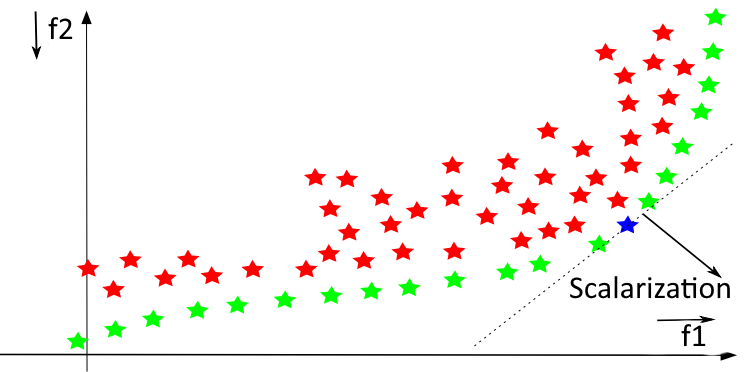
\includegraphics[scale=0.33]{3.png}
\end{center}
\columnbreak
\textbf{Budgeting}: bound the value of one of the losses\\
	$min\{f_1(x)\:|\:f_2(x)\leq \beta_2,x\in X\}$, but which $\beta_2$?
\begin{center}
	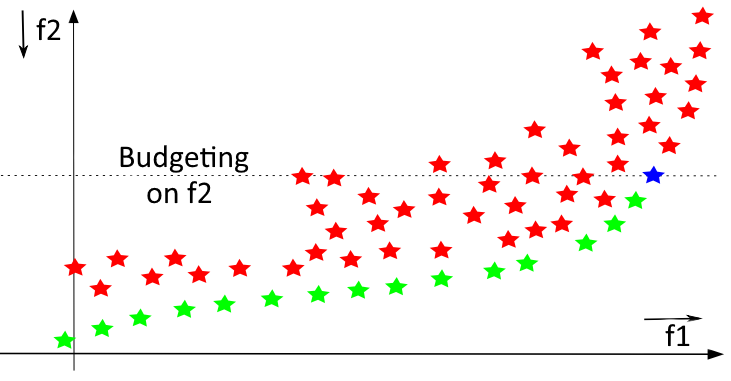
\includegraphics[scale=0.33]{4.png}
\end{center}
\end{multicols}
We will assume that this is done at modelling stage.
\subsection{Optimization is hard}
Even with single-objective, optimization is hard. It's impossible if $f$ has no minimum in $X$, for example $f(x) = x$: if $(P)$ is unbounded below, then $v(P) = -\infty$. Solving $(P)$ is actually at least two different things:
\begin{list}{}{}
	\item finding $x_*$ and \textbf{proving $x_*$ it's optimal} (how?)
	\item constructively \textbf{proving $f$ unbounded below} on $X$ (how?)
\end{list}
It's also impossible if $f_* > -\infty$ but $\not\exists\:x_*$, for example $f(x) = e^x$ or $f(x)=\left\{\begin{array}{l l}
1&\hbox{if }x = 0\\
|x|&\hbox{if }x \neq 0
\end{array}\right.$, but there are plenty of $\epsilon$-approximate solutions ($\epsilon$-optima) $$f(x_\epsilon)\leq f_* + \epsilon\:\:\:\:\forall\:\epsilon>0$$
and on computers $x\in R$ is actually $x\in Q$ with up to 16 digits precision, so approximation errors are unavoidable anyway. Exact algebraic computation is possible but too slow, so ML is actually going the opposite way (float, half, small integers\ldots). And anyway, finding the exact $x_*$ is impossible in general.
%\paragraph{Optimality conditions} If derivative non zero, point no local minimum. Hence $f'(x)=0$ in all local minima but also local maxima as well in saddle.\\
%With $f$ differentiable at $x$ and $x$ local minimum $\Rightarrow \nabla f(x) = 0 \Leftrightarrow$ stationary point ($\not\Leftarrow$)\\
%Theorems proofs breed algorithms: by contradiction $x$ local minimum but $\nabla f(x)\neq 0$. Mathematically speaking, $\exists\:\overline{\alpha} > 0\:|\:\phi(\alpha) < f(x) = \phi(0)\:\:\forall\:\alpha\in[0, \overline{\alpha}]$\\
%SVM are constructed by creating a convex function as stated in the notes.
\paragraph{Optimization need to be approximate} \begin{list}{}{}
	\item \textbf{Absolute gap}: $\{a_i = A(x_i) = f(x_i) - f_*\}$ so $A(x) = f(x) - f_*$ ($\geq 0$)
	\item \textbf{Relative gap}: $\{r_i = R(x_i) = \frac{f(x_i) - f_*}{|f_*|} = \frac{A(x_i)}{|f_*|}\}$ so $R(x) = \frac{f(x) - f_*}{|f_*|} = \frac{A(x)}{|f_*|}$ ($\geq 0$)
\end{list}
The relative gap is useful because $\forall\:\alpha>0$ we have that $(P)\equiv (P_\alpha) = min\{\alpha f(x)\:|\:x\in X\}$, and for the same $x_*$ we have $v(P_\alpha) = \alpha v(P) \Rightarrow$ same $R(x)$, different $A(x)$\\
But in general computing the absolute/relative gap is hard because we don't know $f_*$, which is what we want to estimate. So it's hard to estimate how good a solution is. Could argue that this is the "issue" in optimization: compute an estimate of $f_*$.
\paragraph{Optimization is really hard} Impossible, even, because isolated minima can be anywhere, and restricting to $x\in X=[x_-, x_+]$ with $-\infty<x_-<x_+<+\infty$ doesn't help: still uncountable many points to try. Also $f$ can have isolated downward spike anywhere. Even on $X = [x_-, x_+]$ the spikes can be arbitrarily narrow.
\paragraph{Optimization at least possible} We can impose $X=[x_-,x_+]$ with $D = x_+-x_-<\infty$, meaning with a fixed finite diameter. We can also impose that the $f$'s spikes can't be arbitrarily narrow, so $f$ cannot change too fast $\equiv$ $f$ Lipschitz continuous (L-c) on $X$: $$\exists\: L > 0\:|\:\:\:|f(x) - f(y)| \leq L|x - y|\:\:\:\forall x,y\in X$$
$f$ L-c $\Rightarrow$ doesn't "jump" and one $\epsilon$-optimum can be found with $O(\frac{LD}{\epsilon})$ evaluations by uniformly sampling $X$ with step $\frac{2\epsilon}{L}$. There's a bad news: no algorithm can work in less that $\Omega(\frac{LD}{\epsilon})$, but it's the worst case of $f$ (constant with one spike).\\
The number of steps is inversely proportional to accuracy: just not doable for small $\epsilon$. Dramatically worse with $X\subset R^n$.\\
Also generally $L$ is unknown and not easy to estimate, but algorithms actually require/use it.
\subsection{Local Optimization} Even if I stumble in $x_*$ how do I recognize it? This is the difficult thing. It's simpler to start with a weaker condition: $x_*$ is the local minimum if it solves $min\{f(x)\:|\:f\in X(x_*, \epsilon) = [x_* - \epsilon, x_* + \epsilon]\}$ for some $\epsilon > 0$.\\
Stronger notion: \textbf{strict} local minimum if $f(x_*) < f(y)\:\:\:\forall\:y\in X(x_*,\epsilon) - \{x_*\}$\\
$f$ (strictly) \textbf{unimodal} on X if has minimum $x_* \in X$ and it is (strictly) decreasing on the left $[x_-, x_*]$ and (strictly) increasing on the right $[x_*, x_+]$. If $x_*$, then typically $\exists\:\epsilon>=\:|\:f$ is (strictly) unimodal on $X(x_*,\epsilon)$
Most functions are not unimodal, but they are if you focus on the attraction basin of $x_*$ and restrict there. Unfortunately it's true for every local optimum, they all look the same.
\begin{center}
	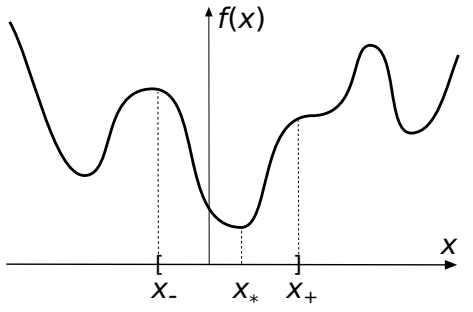
\includegraphics[scale=0.5]{5.png}
\end{center}
Once in the attraction basin, we can restrict it by evaluating $f$ in two points and excluding a part.
\begin{center}
	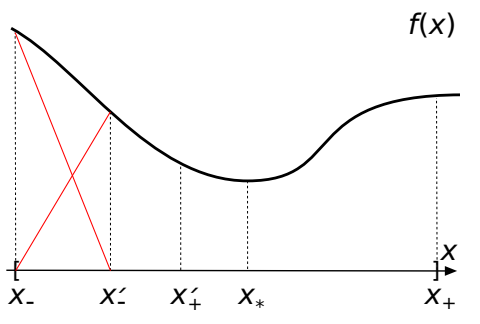
\includegraphics[scale=0.5]{6.png}
\end{center}
How to choose the part so that the algorithm go as fast as possible? Each iteration dumps the left or the right part, don't know which $\Rightarrow$ should be equal $\Rightarrow$ select $r \in (\frac{1}{2}, 1), x'_- = x'_- + (1 - r)D, x'_+ = x_- + rD$\\
Faster if $r$ larger $\Rightarrow$ $r = \frac{D}{2} + \epsilon = x'_\pm = x_- + \frac{D}{2} \pm \epsilon$ but next iteration will have two entirely different $x'_-, x'_+$ to evaluate $f$ on.
\paragraph{Optimally choosing the iterates} A generally powerful concept is to optimize the worst-case behavior $\Rightarrow$ shrink the intervals as quickly as possible.\\
Each iteration dumps either $[x_-, x_-']$ or $[x_+', x_+]$, we don't know which so they should be of equal size $\Rightarrow$ select $r\in (\frac{1}{2},1)$ so that $x_-' = x_- + (1-r)D$ and $x_+' = x_- + rD$\\
$r$ larger $\Rightarrow$ faster convergence, so $r = \frac{D}{2} + \epsilon \Leftrightarrow x_\pm' = x_- + \frac{D}{2}\pm\epsilon$ but next iteration will have two entirely different $x_-', x_+'$ to evaluate $f$ on.\\
So we actually want to minimize function evaluations by reusing the surviving point. $$r : 1 = (1 - r) : r \Leftrightarrow r\cdot r = 1 - r \Leftrightarrow r = \frac{\sqrt{5} - 1}{2} = 0.618 = \frac{1}{g}$$ with $g$ being the golden ratio, $g = \frac{\sqrt{5} + 1}{2} = 1.618 \Rightarrow g = 1 + r = 1 + \frac{1}{g}$\\
Theorems breed algorithms: \textbf{golden ratio search}\\
\begin{lstlisting}[style=myPython]
procedure x = GRS(f, xl, xr, delta)
	xl2 = xl + (1-r)(xr-xl)
	xr2 = xl + r(xr - xl)
	compute f(xl2), f(xr2)
	while (xr - xl > delta):
		if(f(xl2) > f (xr2))
			xl = xl2
			xl2 = x
			x = xr2
			xr2 = xl + r(xr - xl)
			compute f(xr2)
		else:
			xr = xr2
			xr2 = x
			x = xl2
			xl2 = xl + (1-r)(xr-xl)
			compute f(xl2)
\end{lstlisting}
After $k$ iterations, $x_+^k - x_-^k = Dr^k$ stops when $Dr^k \leq \delta$, so when $k = 2\log\frac{D}{\delta}$: exponentially faster, can work with small $\delta$.\\
Asymptotically optimal if no other information is available. $\delta \neq \epsilon$ but $f$ L-c $\Rightarrow A(x^k) \leq \epsilon$ when $k = 2\log\frac{LD}{\epsilon}$\\
First example of linear convergence $A(x^k) \leq Sr^k \leq \epsilon$ with $r < 1$, as fast as a negative exponential $\Rightarrow k \geq \frac{\log\frac{S}{\epsilon}}{\log\frac{1}{r}}$\\\\
$O(\log(\frac{1}{\epsilon}))$ good, but the constant $\rightarrow\infty$ as $r\rightarrow 1$
\paragraph{To make it go faster, give it more information} Two points are needed to see in which direction $f$ is decreasing. If we could see this directly we could make it with one point, faster. Look at the linear function that best locally approximates $f$, trusty old first derivative $f'(x)$: slope of the tangent line to the graph of $f$ in $x$\\
First order model of $f$ at $x$: $$L_x(y)=f'(x)(y-x) + f(x)$$ $L_x(y) \simeq f(y)\:\:\:\:\forall\:y\in[x-\epsilon, x+\epsilon]$ for some small $\epsilon > 0$.\\
$x_*$ local minimum $\Rightarrow f'(x_*) = 0 \Leftrightarrow$ root of $f' \Leftrightarrow$ stationary point. If $f'(x) < 0$ or $f'(x) > 0$, then $x$ is clearly not a local minimum. Hence, $f'(x) = 0$ for the all local minima (hence in the global minimum as well) but this is true for the local maxima (hence global maximum as well), as well in the plateau and saddle points. To tell them apart, look at the second derivative $f''$.
\begin{center}
	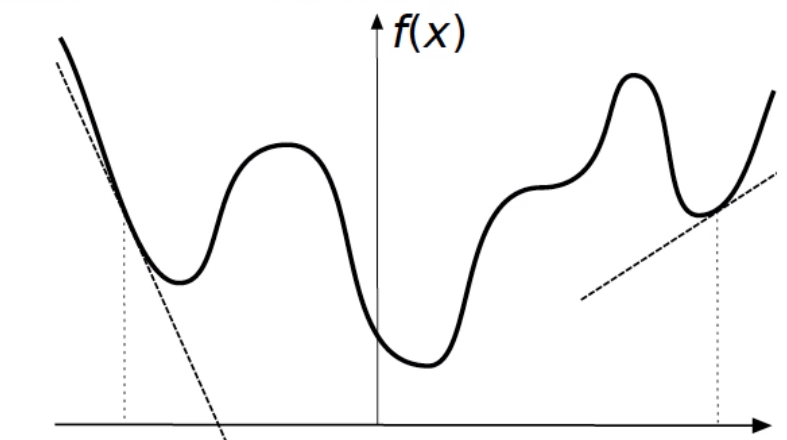
\includegraphics[scale=0.5]{1.png}
\end{center}
In simple cases we get the answer by a closed formula. In $f = bx + c$ linear, if $b > 0$ then the minimum is $x_-$ and maximum is $x_+$, viceversa if $b < 0$. For $f = ax^2 + bx + c$, quadratic, then if $a > 0$ the minimum is min$\{ x_+, max\{x_*, x_-\}\}$ and the maximum is argmax$\{f(x_-), f(x_+)\}$, and viceversa if $a < 0$.\\
Only polynomial whose root have a closed formula (degree 3 and some degree 4), with basically no hope for most trascendental, trigonometric and mixed equations. We need an algorithm for solving non-linear equations.
\paragraph{Dichotomic Search} $f'$ continuous and the intermediate value theorem gives that $$f'(x_-) < 0 \wedge f'(x_+) > 0 \Rightarrow \exists\:x\in[x_-, x_+]\:|\: f'(x) = 0$$
Theorems breed algorithms $\rightarrow$ \textbf{Dichotomic Search}.
\begin{lstlisting}[style=myPython]
procedure x = DS(f, xl, xr, eps)
	while (true) do:  # invariant: df(xl)<-eps, df(xr)>eps
		x = in_middle_of(xl, xr)
		compute df(x)
		if (abs(df(x)) <= eps): break
		if (df(x) < 0):
			xl = x
		else:
			xr = x
\end{lstlisting}
With \texttt{df} meaning $f'$\\
For \texttt{in\_middle\_of(xl, xr)} the obvious choice is \texttt{return (xl + xr)/2;}. We have linear convergence with $\gamma = 0.5 < 0.618 \Rightarrow k = 1.45\log(\frac{LD}{\epsilon}) < 2 \log(\frac{LD}{\epsilon})$\\
The condition $f'(x_-) < -\epsilon, f'(x_+) > \epsilon$ is important. What if is not satisfied? Obvious solution, moving the interval more and more to the right until the derivative is possible. %TODO
The same in reverse of $x_-$ with $\Delta x = -1$. This works in practice for all "reasonable" functions. Works if $f$ coercive ($\lim_{|x| \to \infty} f(x) = \infty$)\\
\begin{list}{}{}
	\item $f' \in C^0 \Leftrightarrow f \in C^1 \Leftrightarrow$ continuously differentiable $\Rightarrow f\in C^0$
	\item $f'' \in C^0 \Leftrightarrow f\in C^2 \Leftrightarrow f' \in C^1 \Rightarrow f' \in C^0 \Rightarrow f \in C^1 \Rightarrow f \in C^0$
	\item $f \in C^1$ globally L-c on $X \Rightarrow |f'(x)| \leq L \forall\: x \in X$
\end{list}
\paragraph{Extreme value theorem} $f \in C^0$ on $X = [x_-, x_+]$ finite $\Rightarrow$ max$\{f(x)\:|\: x\in X\} < \infty$, min$\{f(x)\:|\: x\in X\} > -\infty$\\\\
$f\in C^1$ on $X$ finite $\Rightarrow f$ globally L-c on $X$\\
Best possible case is $f\in C^2$ on finite $X\Rightarrow$ both $f$ and $f'$ globally L-c on $X$
\paragraph{Fastest local optimization} Interpolation, for improving the dichotomic search. Choosing $x$ "right in the middle" is the dumbest possible approach, because we know a lot about $f$: $f(x_-), f(x_+), f'(x_-), f'(x_+)\ldots$. So let's use that, by constructing a model of $f$ based on known information. Much better choosing $x$ close to $x_*$.\\
But remember that \textbf{the model is an estimate}, so never completely trust the model, but regularize, stabilize\ldots in this case, the minimum guaranteed decrease is with $\sigma < 0.5$, and the worst case is linear convergence with $r = 1 - \sigma$, but hopefully is much faster than that when the model is "right".
\pagebreak
\subsection{Measuring algorithms speed} Given the sequences \begin{list}{}{}
	\item $\{x_i\}$
	\item $\{d_i = |x_i - x_*|\}$
	\item $\{f_i = f(x_i)\}$
	\item $\{a_i = A(x_i) = f(x_i) - f_*\}$ absolute gap
	\item $\{r_i = R(x_i) = \frac{f(x_i) - f(x)}{|f_*|} ) \frac{A(x_i)}{|f_*|}\}$ relative gap
\end{list}
We have convergence when $\{a_i\} \rightarrow 0, \{r_i\} \rightarrow 0 \Leftarrow \{d_i\} \rightarrow 0$ (but $\not\Rightarrow)$, but how rapidly? \textbf{Rate of convergence}
$$\lim_{i\to\infty} \left(\frac{f_{i+1} - f_*}{f_i - f_*}\right)^p = \lim_{i\to\infty} \left(\frac{a_{i+1}}{a_i}\right)^p = \lim_{i\to\infty} \left(\frac{r_{i+1}}{r_i}\right)^p = r$$
\begin{list}{}{}
	\item[$p = 1$]\begin{list}{}{}
		\item $r = 1\Rightarrow$ sublinear \begin{list}{}{}
			\item $\frac{1}{i} \Rightarrow k \in O(\frac{1}{\epsilon})$ (bad)
			\item $\frac{1}{i^2} \Rightarrow k \in O(\frac{1}{\sqrt{\epsilon}})$ (a bit better)
			\item $\frac{1}{\sqrt{i}} \Rightarrow k \in O(\frac{1}{\epsilon^2})$ (horrible)
		\end{list}
		\item $r < 1\Rightarrow$ linear, $r_i \rightarrow i \in O(\log(\frac{1}{\epsilon})$, good unless $r = 1$
	\end{list}
	\item[$p \in (1,2)$] $p = 1, r = 0\Rightarrow$ superlinear
	\item[$p = 2$] $r > 0\Rightarrow$ quadratic, best we can reasonably hope for\\
	$\frac{1}{2^{2^i}} \Rightarrow i \in O(\log(\log(\frac{1}{\epsilon})))$, which is basically $O(1)$: the number of correct digits double at each iteration
\end{list}
\paragraph{Improving dichotomic search} Quadratic interpolation has superlinear convergence if started "close enough".\\
$f\in C^3, f'(x_*) = 0 \wedge f''(x_*)\neq 0 \Rightarrow \exists\:\delta > 0\:|\:x_0 \in [x_* - \delta, x_* + \delta] \Rightarrow \{x_i\} \rightarrow x_*$ with $p = \frac{1 + \sqrt{5}}{2}$ exponent of superlinear convergence.\\$x_0$ is the starting point of the algorithm.\\\\
Four conditions $\Rightarrow$ can fit a cubic polynomial and use its minima. Theoretically pays: quadratic convergence ($p = 2$) and seems to work well in practice.
\paragraph{Newton's method} More derivatives, so same information with less points. First order model of $f'$ at $x_i$ $$L_i'(x) = L_{x_i}'(x) = f'(x_i) + f''(x_i)(x-x_i)\simeq f'(x)$$ and solve $L'_i(x) = 0 \simeq f'(x) = 0 \Rightarrow x = x_i-\frac{f'(x_i)}{f''(x_i)}$
\begin{lstlisting}[style=myPython]
procedure x = NM(f, x, eps)
	while (abs(df(x)) > eps):
		x = x - (df(x)/ddf(x))
\end{lstlisting}
With \texttt{df} meaning $f'$ and \texttt{ddf} meaning $f''$.\\
Alternatively construct a second order model $$Q_i(x) = Q_{x^i}(x) = f(x^i) + f'(x^i)(x - x^i) + f''(x^i)\frac{(x - x^i)^2}{2}$$ and then minimize it.\\\\
Numerically delicate: what if $f''(x) \simeq 0$? Converges (at all) only if started close enough to $x_*$.\\
If we get within a short enough distance $\delta$, then it will converges extremely fast with $p = 2$. Mathematically, $f\in C^3, f'(x_*) = 0 \wedge f''(x_*)\neq 0\Rightarrow \exists\:\delta>0\:|\:x_0\in[x_*-\delta, x_*+\delta]\Rightarrow \{x_i\} \rightarrow x_*$ with $p = 2$.
\pagebreak
\subsection{Global optimization} Unless strong assumptions are made, we can't say much about global optimization.\\
The obvious one would be unimodal, but not easy to verify/construct. Workable alternative: $f$ convex ($\Rightarrow$ unimodal).
\paragraph{Convexity} Convex means that $f'$ monotone non decreasing and $f'' \geq 0$. But convexity $\not\Rightarrow C^1$. Some functions are convex and a few operators preserve convexity. Many models are purposely constructed convex $\Rightarrow$  \textbf{Spatial Branch-and-Bound approach}: sift through all $X = [x_-, x_+]$ using clever guide, convex lower approximation \underline{$f$} of nonconvex $f$ on $X$.
\begin{center}
	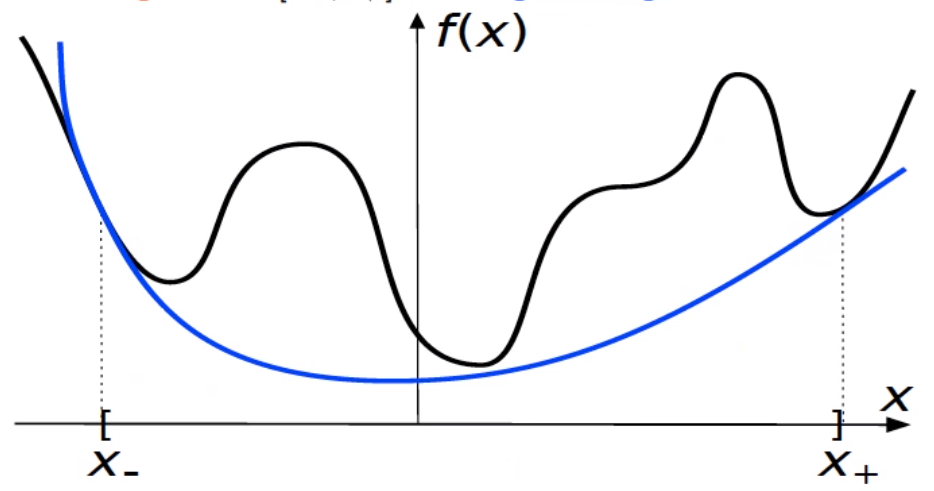
\includegraphics[scale=0.5]{2.png}
\end{center}
"Easily" find local $\equiv$ global minimum $\overline{x}$ giving \underline{$f$}$(\overline{x}) \leq f_* \leq f(\overline{x})$. If the gap $f(\overline{x}) - \underline{f}(\overline{x})$ is too large, we partition $X$ and iterate. If on some partition $\underline{f}(\overline{x}) \geq$ best $f$-value so far, then that partition is killed.\\
In the worst case, exponential complexity because you keep dicing and slicing $X$. But it is exponential in practice too. It depends on how much non-convex $f$ is and how good of a lower approximation $\underline{f}$ is. A cleverer approach is carefully choosing the non-convexities.
%end 1-first steps.pdf
\section{Unconstrained optimization}
From now on we'll use $f:R^n\rightarrow R$, i.e. $f(x_1,x_2,\ldots,x_n) = f(x)$ with $x = [x_i]_{i=1}^n = [x_1,\ldots,x_n]\in R^n$. Note that $R^n = R\times R \times\ldots\times R$, which is \textbf{exponentially larger} than $R$.\\
$I = [x_-, x_+], X = I\times I \times\ldots\times I$ hypercube (or hyperrectangle if intervals are disequal).\\\\
We need $f$ to be L-c, and sadly no algorithm can work in less than $\Omega((\frac{LD}{\epsilon})^n)$. \textbf{Curse of dimensionality}: not really doable unless $n = 3, 5, 10$ tops. Can make to $O((\frac{LD}{\epsilon})^n)$, with multidimensional grid and small enough step (standard approach to hyperparameter optimization). If $f$ analytic, clever B\&B can give global optimum. If $f$ black-box (typically, no derivatives), many heuristics can give good solutions, probably not optimal.
\subparagraph{Unconstraint global optimization} If $f$ is convex, then global $\equiv$ local which is much better: most (but not all) convergence results are dimension independent and if there's dependence it is not exponential. Doesn't mean that all local algorithms are fast: speed may be low (badly linear), cost of $f$ or derivatives computation increases with $n$ dimension (for large n even $O(n^2)$ may be too much) and some dependency on $n$ may be hidden in $O(\:)$ constraints. Yet, large scale optimization can be done.
\paragraph{Notation}\begin{list}{}{}
	\item \textbf{Scalar product} $\langle x,y\rangle = x^Ty = \sum_{i=1}^n x_iy_i = x_1y_1+\ldots+x_ny_n$
	\item \textbf{Norm} $||x|| = \sqrt{x_1^2+\ldots+x_n^2} = \sqrt{\langle x,x\rangle}$
	\item \textbf{Distance} $d(x,y) = ||x-y|| = \sqrt{(x_1-y_1)^2+\ldots+(x_n-y_n)^2}$
	\item \textbf{Ball} with center $r\in R^n$ and radius $r > 0$ is $B(x,r) = \{y\in R^n\:|\:||y-x||\leq r\}$
\end{list}
Usually $f:D\rightarrow R$ with $D = dom(f)$ domain of $f$ which may not be all $R^n$, but usually ok to ignore $dom(f)$ and assume $f(x)=\infty$ for $x\not\in D$
\begin{list}{}{}
	\item \textbf{Graph} of $f$ lives in $R^{n+1}$: $gr(f) = \{(f(x),x)\:|\:x\in R^n\}$
	\item \textbf{Epigraph} of $f$ lives in $R^{n+1}$: $epi(f)=\{(v,x) \in R^{n+1}\:|\:v\geq f(x)\}$
	\item \textbf{Level set} at value $v$: $L(f,v)=\{x\in R^n\:|\:f(x)=v\}$
	\item \textbf{Sublevel set} at value $v$: $S(f,v)=\{x\in R^n\:|\:f(x)\leq v\}$
\end{list}
We have that $x_* \in S(f,v)\:\:\:\forall\:v\geq f_*$ and $S(f,v) = \emptyset\:\:\:\forall\:v<f_*$

\paragraph{Tomography} $f:R^n \rightarrow R$ with $x\in R^n$ origin and $d\in R^n$ direction. You can define $\phi_{x,d}(\alpha) = f(x + \alpha d): R \rightarrow R$ \textbf{tomography} of $f$ from $x$ along $d$.\\
$\phi_{x,d}$ can always be pictured, but there are infinitely many of them: which $x,d$?\begin{list}{}{}
	\item $||d||$ only changes the scale: $\phi_{x,\beta d}(\alpha) = \phi_{x,d}(\beta \alpha)$ so often convenient to use normalised direction ($||d|| = 1$)
	\item Simplest case: restriction along $i$-th coordinate\\
	$f_x^i(\alpha) = f(x_1,\ldots,x_{i-1},\alpha,x_{i+1},\ldots,x_n) = \phi_{0,u^i}(\alpha)$ with $||u^i|| = 1$
	\item When $x,d$ clear from context, then $\phi(\alpha)$
\end{list}
\paragraph{Simple Functions} \begin{list}{}{}
	\item \textbf{Linear} $f(x) = \langle b,x\rangle + c, b \in R^n, c\in R$\\
	Tomography $f(x) = \langle b,x\rangle, x = 0, ||d||=1$: $\phi(\alpha) = \alpha\langle b, d\rangle = \alpha||b||cos(\theta)$\\
	Plotting this gives a line, increasing because "$b$ same direction as $d$", more collinear $\Rightarrow$ steeper. Collinear means steepest line, less collinear means less steap. 90° angle means a flat line. Decreasing if opposite directions.\\
	min $f(x)$ when $\not\exists\:x_*$ if $b \neq 0$ ($\Rightarrow \exists\: d\:|\:\langle b,d\rangle \neq 0$), $\forall\:x$ if $b = 0$
	\item \textbf{Quadratic} with fixed $Q\in R^{n\times n}, q\in R^n$ we have $f(x) = \frac{1}{2}x^TQx + qx$. If $q=0$ (no linear term), then \textbf{homogeneous quadratic}.\\
	Tomography $\phi(\alpha) = f(\alpha d) = \alpha^2(d^TQd)\Rightarrow$ sign and steepness depend on $d^TQd$, so we need to know about signs of $d^TQd$. Steeper when $d$ along one axe, least steep when $d$ along the other axe and intermediate steepness when "in between". Again, steeper along the opposite of one axe and least steep along the opposite of the other axe.\\
	With $q\neq 0$ but $Q$ nonsingular then $\lambda_i\neq 0\:\:\:\forall\:i$, then $f(x)=\frac{1}{2}(x-x_*)^TQ(x-x_*) [+c]$ for $x_* = -Q^{-1}q$ and $x_* \neq 0$ center of the level sets (which shapes are determined by the eigenvalues).\\
	$y = x - x_*, f_*(y) = y^TQy [+c]$
\end{list}
\paragraph{Directional/partial derivatives} The directional derivative of $f:R^n\rightarrow R$ at $x\in R^n$ along the direction $d\in R^n$ is $$\frac{\partial f}{\partial d}(x) = \lim_{t\to 0}\frac{f(x+td) - f(x)}{t} = \phi_{x,d}'(0)$$
How can $\phi_{x,d}'(0)$, the derivative of the $(x,d)$-tomography (in 0), be computed? A special case is $\frac{\partial f}{\partial d}(x)$, partial derivative of $f$ with respect to $x_i$ at $x\in R^n$, easy to compute by just treating $x_j$ for $j\neq i$ as constants.\\
The \textbf{gradient} is the column vector of all partial derivatives $$\nabla f(x) = \left[\begin{array}{c}
\frac{\partial f}{\partial x_1}(x)\\
\vdots\\
\frac{\partial f}{\partial x_n}(x)
\end{array}\right]$$
$$f(x) = \langle b,x\rangle \Rightarrow\nabla f(x) = b$$
$$f(x) = \frac{1}{2}x^TQx + qx \Rightarrow\nabla f(x) = Qx + q$$
$f$ differentiable at $x$ if $\exists$ linear function $\psi(h) =\langle b,h\rangle + f(x)$ such that $$\lim_{||h||\to 0}\frac{|f(x+h) - \psi(h)}{||h||} = 0$$ $$\Rightarrow \psi(0) = f(x) \Rightarrow c = f(x)$$
$\psi$ is equivalent to the first order model of $f$ at $x$, the error of this equivalence vanishes faster than linearity. So $f$ differentiable at $x\Rightarrow b = \nabla f(x)$ and\begin{list}{}{}
	\item $\Rightarrow \frac{\partial f}{\partial x_i}(x)$ exists for every $i$ (but $\Leftrightarrow$ not true)
	\item $\Rightarrow$ first order model of $f$ at $x$ is $L_x(y) = \nabla f(x)(y-x)$
\end{list}
$f$ differentiable $\Rightarrow$ all relevant objects in $R^{n+1}$ and $R^n$ are smooth. If $f$ is non differentiable $\Rightarrow$ kinks appear and things break,
\paragraph{Jacobian} Given a vector-valued function $f:R^n\rightarrow R^m$, $f(x) = [f_1(x), f_2(x),\ldots,f_m(x)]$, the partial derivatives are the same with extra index $$\frac{\partial f_j}{\partial x_i}(x) = \lim_{t\rightarrow 0}\frac{f_j(x_1,\ldots,x_{i-1},x_i+t,x_{i+1},\ldots,x_n) - f_j(x)}{t}$$
The \textbf{Jacobian} is the matrix of all $mn$ partial derivatives
$$Jf(X) = \left[ \begin{array}{c c c}
\frac{\partial f_1}{\partial x_1}(x) & \ldots & \frac{\partial f_1}{\partial x_n}(x)\\
\vdots&\ddots&\vdots\\
\frac{\partial f_m}{\partial x_1}(x) & \ldots & \frac{\partial f_m}{\partial x_n}(x)\\
\end{array}\right] = \left[\begin{array}{c}
\nabla f_1(x)^T\\\vdots\\\nabla f_m(x)^T
\end{array}\right]$$
A $m\times n$ matrix with gradients as rows.
\paragraph{Hessian} The $\frac{\partial f}{\partial x_i}:R^n\rightarrow R$ have partial derivatives themselves. \textbf{Second order partial derivative}, just do it twice $$\frac{\partial^2 f}{\partial x_i \partial x_j}$$ $$\frac{\partial^2 f}{\partial x_i \partial x_i}=\frac{\partial^2 f}{\partial x_i^2}$$
So $\nabla f(x) : R^n \rightarrow R^n$ have a Jacobian and it's called \textbf{Hessian} of $f$ at $x$
$$\nabla^2 f(x) = J\nabla f(x) = \left[ \begin{array}{c c c c}
\frac{\partial^2 f}{\partial x_1^2}(x) & \frac{\partial^2 f}{\partial x_2\partial x_1} & \ldots & \frac{\partial^2 f}{\partial x_n\partial x_1}(x)\\
\vdots&\ddots&\ddots&\vdots\\
\frac{\partial^2 f}{\partial x_1\partial x_n}(x) & \frac{\partial^2 f}{\partial x_2\partial x_n}(x) & \ldots & \frac{\partial^2 f}{\partial x_n^2}(x)\\
\end{array}\right]$$
Requires $O(n^2)$ to store and at least $O(n^2)$ to compute, unless sparse.\\
$f(x) = \frac{1}{2}x^TQx + qx \Rightarrow \nabla^2 f(x) = Q$\\
Second order model = first order model plus second order term (better)
$$Q_x(y) = L_x(y) + \frac{1}{2}(y-x)^T\nabla^2f(x)(y-x)$$
\subparagraph{Theorem} $\exists\:\delta>0\:|\:\forall\:y\in B(x, \delta)$ we have that $\frac{\partial^2 f}{\partial x_j\partial x_i}(y)$ and $\frac{\partial^2 f}{\partial x_i\partial x_j}(y)$ exist and are continuous in $x$\begin{list}{}{}
	\item $\Rightarrow \frac{\partial^2 f}{\partial x_j\partial x_i}(y) = \frac{\partial^2 f}{\partial x_i\partial x_j}(y) \Leftrightarrow \nabla^2 f$ symmetric
	\item $\Rightarrow$ all eigenvalues of $\nabla^2 f(x)$ are real
\end{list}
With $f\in C^2$ we have $\nabla^2 f(x)$ continuous everywhere, so symmetric everywhere. $C^2$ is the best class for optimization.
\subsection{Optimality conditions}
$f$ differentiable at $x$ and $x$ local minimum $\Rightarrow \nabla f(x) = 0 \equiv$ stationary point ($\not\Leftarrow$): to tell them apart we need to look at the curvature of $f$. If $f$ quadratic I wold know, looking at the eigenvalues of $Q = \nabla^2 f(x)$, so we could approximate $f$ with a quadratic function: the second order model $Q_x(y) = L_x(y) + \frac{1}{2}(y-x)^T\nabla^2f(x)(y-x)$\\
$\nabla Q_x(x) = \nabla L_x(x) = \nabla f(x) \Rightarrow \nabla Q_x(x) = 0$, otherwise not minimum. Meaning that in a local minimum there cannot be directions of negative curvature, $\nabla^2 f(x) \geq 0 \Leftrightarrow x$ (global) minimum of $Q_x$.\\
Another condition necessary and almost sufficient: $f\in C^2$.
%end 2-uncostrained optimality.pdf
\subsection{Gradient Methods}
\paragraph{Multivariate optimization algorithms} These are iterative procedures: start from an initial guess $x_0$ and compute some process $x_i \longrightarrow x_{i+1}$ to get a \textbf{sequence} $\{x_i\}$ that \textbf{should go towards an optimal solution}. $\{x_i\}\rightarrow x_*$ is one option, the best one, but not the only possibility.\\
At least $\{f_i = f(x_i)\} \rightarrow f_*$: \textbf{minimizing sequence}, and clearly $\{x_i\}\rightarrow x_* \Rightarrow \{f_i\}$ minimizing sequence, but $\not\Leftarrow$\\
Two general forms of the process $x_{i+1} = x_i + \alpha_id_i$:
\begin{list}{}{}
	\item \textbf{Line search}: first choose $d_i\in R^n$ (\textbf{direction}), then choose $\alpha_i\in R$ (\textbf{step size} $\equiv$ learning rate in ML)
	\item \textbf{Trust region}: first choose $\alpha_i\in R$ (\textbf{trust radius}), then $d_i$
\end{list}
The crucial concept is that the \textbf{model} $f_i \simeq f$ is used to construct $x_{i+1}$ from $x_i$
\paragraph{First order model $\equiv$ gradient method} The first order model is the simplest model $$L_i(x) = L_{x_i}(x) = f(x_i) + \nabla f(x_i)(x-x_i)$$ Idea: $x_{i+1} \in argmin\{L_i(x) : x\in R^n\} = \emptyset$, $L_i$ unbounded below on $R^n$\\
It shouldn't move too far from $x_i$, $L_i$ is only "good" as $\alpha_i\rightarrow 0 \Rightarrow d_i = argmin\{\lim_{t\to 0} \frac{f(x+td)}{t}\} = -\nabla f(x_i) =$ steepest descent direction.\\
$\frac{\partial f}{\partial d_i}(x_i) < 0$ but $\frac{\partial f}{\partial d_i}(x_i + \alpha d_i)$ likely $> 0$ when $\alpha$ groes $\Rightarrow f$ grows instead of decreasing $\Rightarrow$ very long steps are bad unless $f_* = -\infty$. Very short steps are bad too: $f$ decreases, but very slowly.
\paragraph{Step selection} The issue is to find the Goldilocks Step $\alpha_i$ efficiently (a few function evaluations). Two extreme strategies:
\begin{list}{}{}
	\item \textbf{Fixed Stepsize} (FS): $\forall\:i\:\:\:\alpha_i = \overline{\alpha}$ (how is chosen?)\\
	Most inexpensive.
	\item \textbf{(Exact) Line Search} (LS): $\alpha_i\in argmin\{f(x_i+\alpha d_i\}\:|\:\alpha\geq 0\}$\\
	Most expensive but may converge faster.
\end{list}
Of course, something in the middle is better. $\phi'_i$ low-degree polynomial $\Rightarrow f(x_i+\alpha d_i) = \phi_{x_i,d_i}(\alpha) = \phi_i(\alpha)$
\paragraph{Gradient for quadratic functions} $f(x) = \frac{1}{2}x^TQx + qx$ with $Q\geq 0$ otherwise $f$ is unbounded below. $x_*$ solves $Qx = -q$ if it exists, which is linear algebra but the linear system requires at most $O(n^3)$ while computing $d_i = -\nabla f(x_i) = -Qx_i - q$ is $O(n^2)$\\
Line search is easy, $O(n^2)$ with $\alpha_i = \frac{||d_i||^2}{d_i^TQd_i}$
\begin{lstlisting}[style=myPython]
procedure x = SDQ(Q, q, x, eps):
	while (||nablf(x)||>eps):
		d = -nablf(x)
		alpha = ||d||^2/dT*Q*d
		x = x + alpha*d
\end{lstlisting}
With \texttt{nablf} being $\nabla f$
\subparagraph{Analysis} Never obvious because we have to use properties of $x_*$ which is unknown, but in this case there's a nifty trick
$$f_*(x) = \frac{1}{2}(x-x_*)^TQ(x-x_*) = f(x) - f_*(x) = A(x)$$
for which, with $Q$ positive definite $$A(x_{i+1}) = \left(1-\frac{||d_i||^4}{(d_i^TQd_i)(d_i^TQ^{-1}d_i)} \right)A(x_i)$$
This becomes linear convergences ($\lambda_1,\lambda_{n}$ being respectively the max and min eigenvalues of $Q$)
\begin{list}{}{}
	\item Simple $A(x_{i+1}) \leq (1-\frac{\lambda_n}{\lambda_1})A(x_i)$
	\item Elaborated $A(x_{i+1}) \leq \frac{\lambda_1 - \lambda_n}{(\lambda_1 - \lambda_n)^2}A(x_i)$
\end{list}
The good news is that $n$ doesn't appear, it's \textbf{dimension-independent} so doable for very large scale machine learning. The bad news is that $r\rightarrow 1$ as conditioning of $Q = \frac{\lambda_1}{\lambda_n}\rightarrow\infty$
\paragraph{When linear convergence may not be enough} The convergence is fast if $\lambda_1\simeq \lambda_n$ (one iteration for $||x||^2$) and rather slow if $\lambda_1 >> \lambda_n$. Intuitively, the algorithm zig-zags a lot when level sets are very elongated. Another bad news is that there may be an "hidden dependency": $\lambda_1$ and $\lambda_n$ may depend on $n$ and $\frac{\lambda_1}{\lambda_n}$ may grow as $n\rightarrow\infty$.\\
Let's extend it to every function.
\subsubsection{Gradient methods for general functions}
Given $f$ a general nonlinear function, the algorithm is almost the same:
\begin{lstlisting}[style=myPython]
procedure x = SDQ(f, x, eps):
	while (||nablf(x)||>eps):
		d = -nablf(x)
		alpha = stepsize(f, x, d)
		x = x + alpha*d
\end{lstlisting}
\texttt{stepsize} is the crucial part: FS or (inexact) LS. Need to avoid two opposite problems:
\begin{list}{}{}
	\item Scylla: $\alpha_i$ not too large to avoid $f(x_{i+1}) > f(x_i)$
	\item Charybdis: $\alpha_i$ not too small to avoid stalling
\end{list}
With $\frac{\partial f}{\partial d_i}(x_i)<0$ hence $\alpha_i\rightarrow 0$ we avoid Scylla but may hit Charybdis.\\
\texttt{stepsize(f, x, d)} $= LS(\phi_{x,d}, [0,\infty], \epsilon')$ is attractive but $\epsilon' = 0$ in general is not possible: how to choose it? Depends on the stopping criterion in $LS()$, let's assume $|\phi_{x,d}(\alpha)| \leq \epsilon'$. A fundamental property is $$\phi'_i(\alpha) = \frac{\partial f}{\partial d_i}(x_i + \alpha d_i) = \langle\nabla f(x_i+\alpha d_i), d_i\rangle$$
$$\Rightarrow |\phi_i'(\alpha_i)| = |\langle d_i, \nabla f(x_{i+1})\rangle| = |\langle \nabla f(x_i),\nabla f(x_{i+1})\rangle|$$
The good news is that only an approximate stationary point of $\phi_i$ is needed, no global minimum (and not even a local minimum, can be a local maximum or a saddle point) $\Rightarrow f$ convex/unimodal is not needed. Also we can prove that the algorithm works with $\epsilon' = \epsilon ||\nabla f(x_i)||$\\
A bad news is that the LS should become more accurate as the algorithm proceeds, and the LS can be very approximate ("far from $x_*$").\\
Usually works well in practice with arbitrary fixed $\epsilon'$
\paragraph{Notes on the stopping criterion} One would want $A(x_i)<\epsilon$ or $R(x_i) < \epsilon$ as stopping criterion, the issue is that $f_*$ is often unknown and cannot be used online. We need a lower bound $\underline{f} \leq f_*$, tight at least towards termination, but in general there are no good $\underline{f}$ available because good estimates of $f_*$ are hard to get.\\
We can use $||\nabla f(x_i)||$ as proxy of $A(x_i)$ (small $\Rightarrow$ small) but the exact relationship is hard to assess, so choosing $\epsilon$ is not obvious.\\
Sometimes we use a relative stopping condition $||\nabla f(x_i)||\leq \epsilon||\nabla f(x_0)||$, and sometimes $||\nabla f||$ has some meaning that can be used. Sometimes, we don't really care is $A(x_i)$ or $R(x_i)$ are small (machine learning).
\paragraph{Efficiency} The efficiency is basically the same.\\
With $f\in C^2, x_*$ local minimum such that $\nabla^2f(x_*)$ positive definite, exact LS $\{x_i\}\rightarrow x_* \Rightarrow \{f_i\}_{i\geq k}\rightarrow f_*$ linearly for large enough $k$, with $r = \frac{\lambda_1 - \lambda_n}{\lambda_1 + \lambda_n}^2$ with $\lambda_1,\lambda_n$ those of $\nabla^2 f(x_*)$\\
The result can be extended to inexact LS with $r\simeq 1-\frac{\lambda_n}{\lambda_1}$ (worse), with "$\simeq$" depending on LS parameters.
\subsubsection{Fixed Stepsize}
With $\alpha_i = \overline{\alpha}$ for each $i$ it's much simpler but also rigid. Easier to avoid Charybdis: $\sum_{i=1}^\infty \alpha_i = \infty$\\
Yet $d_i = -\nabla f(x_i) \Rightarrow$ one wants $\{||d_i||\}\rightarrow 0$, so care is still required. We also have that $\alpha_i\rightarrow 0$ surely avoid Scylla, but it's not possible here.\\
The fundamental trick is $d_i = -\nabla f(x_i) \Rightarrow ||x_{i+1} - x_i||$ automatically changes along iterations even if $\alpha_i$ is fixed.\\
$d_i = \frac{-\nabla f(x_i)}{||\nabla f(x_i)||} \equiv ||d_i|| = 1$ would necessarily require $\alpha_i \rightarrow 0$, yet $f$ varies very rapidly so only very short $\alpha_i$ are possible. It's crucial to bound how rapidly $f$ changes.
\paragraph{L-smoothness} $$f \hbox{ L-smooth }\Rightarrow \phi(\alpha) \leq \phi(0) + ||\nabla f(x)||^2\left(\frac{L\alpha^2}{2-\alpha}\right)$$
Powerful general idea: find $\alpha$ giving the best worst-case improvement, meaning $v(\alpha) = \frac{L\alpha^2}{2-\alpha}, \alpha_* = \frac{1}{L}$ (constant!), $v(\alpha_*) = -\frac{1}{2L}$ hence $$f(x_{i+1}) - f(x_i) \leq -\frac{||\nabla f(x_i)||^2}{2L}$$ Can't do better if you trust the quadratic bound (which you should not).\\
The error decreases sublinearly: a term is subtracted to $a_i$ rather than multiplied $a_{i+1} = f(x_{i+1}) - f_* \leq a_i - \frac{||\nabla f(x_i)||^2}{2L}$\\
In fact $a_i\leq \frac{2L||x_0 - x_*||^2}{i+3} \Rightarrow i\geq O(\frac{LD^2}{\epsilon})$ (note that the initial point matters)\\
However we used $Q$ nonsingular $\Leftrightarrow \lambda_n > 0$, which does make a difference.
\paragraph{Stronger forms of convexity}
$f$ convex means that $\forall\:x,y\in R^n$ we have $$\alpha f(x) + (1-\alpha)f(y)\geq f(\alpha x+ (1-\alpha)y)\:\:\:\:\forall\:\alpha\in[0,1] \Leftrightarrow f(y)\geq f(x) + \langle \nabla f(x), y-x\rangle$$
\textbf{Strictly} convex means $$\alpha f(x) + (1-\alpha)f(y)> f(\alpha x+ (1-\alpha)y)\:\:\:\:\forall\:\alpha\in[0,1] \Leftrightarrow f(y)> f(x) + \langle \nabla f(x), y-x\rangle$$
Quadratic with $\lambda_n > 0$ more than that: it grows at least as fast as $\lambda_n||x||_2^2$, meaning \textbf{strongly convex modulus $\lambda_n$} $\equiv \lambda_n$-convex.\\
$f$ \textbf{strongly convex modulus $\tau > 0$} ($\tau$-convex) if $f(x)-\frac{\tau}{2}||x||_2^2$ is convex $\Leftrightarrow$ $$\alpha f(x) + (1-\alpha)f(y)\geq f(\alpha x+ (1-\alpha)y)+\frac{\tau}{2}\alpha(1-\alpha)||y-x||^2\:\:\:\:\forall\:\alpha\in[0,1] \Leftrightarrow$$ $$\Leftrightarrow f(y)> f(x) + \langle \nabla f(x), y-x\rangle+\frac{\tau}{2}||y-x||^2 \Leftrightarrow\nabla^2 f(x) \succeq \tau I$$
$f \in C^2,$ $L$-smooth and $\tau$-convex $\equiv \tau I \preceq \nabla^2 f\preceq LI \equiv \tau \leq \lambda_n \leq \lambda_1 \leq L$, eigenvalues of $\nabla^2 f$ are bounded both below and above.
\paragraph{Convergence rate with strong convexity} Minimize on $x$ both sides independently $$f(x_*)\geq f(x_i) - \frac{||\nabla f(x_i)||^2}{2\tau} \Rightarrow ||\nabla f(x_i)||^2\geq 2\tau(f(x_i)-f(x_*))$$
"If $a_i = f(x_i) - f_*$ is large then the gradient must also be large."\\
$L$-smooth $\Rightarrow a_{i+1}\leq a_i - \frac{||\nabla f(x_i)||^2}{2L} \Rightarrow a_{i+1}\leq a_i(1-\frac{\tau}{L})$\\
A small difference in $f$ makes a big difference in convergence $\Rightarrow$ properties of $f$ more important than the algorithm.
\subsubsection{Inexact Line Search}
\paragraph{Armijo} If FS works, then any rough LS also should work provided that $f_i$ decreases enough.\\
The \textbf{Armijo condition} is $0 < m_1 < 1$
\begin{list}{}{}
	\item[$(A)$] $\phi(\alpha)\leq \phi(0)+m_1\alpha\phi'(0)$
\end{list}
$\alpha \rightarrow 0$ satisfies $(A)$. But if we avoid Charybdis then we "converge".\\
$\alpha_i\geq \overline{\alpha} > 0$ and $(A)$ holds $\forall\:i\Rightarrow$ either $\{f_i\}\rightarrow -\infty$ or $\{||\nabla f(x_i)||\}\rightarrow 0$\\
All accumulation points (if any) of $\{x_i\}$ are stationary. The proof: assume $-\phi_i'(0) = ||\nabla f(x_i)||^2\geq \epsilon > 0$ and $(A)$ hold $\forall\:i\Rightarrow$ $$f_{i+1} \leq f_i + m_1\alpha_i\phi_i'(0)\leq f_i - m_1\overline{\alpha}\epsilon \Rightarrow f_i \leq f_0 - m_1\overline{\alpha}\epsilon \Rightarrow \{f_i\}\rightarrow -\infty$$ Don't even need $\alpha_i\geq \overline{\alpha} > 0$, just $\sum_{i=1}^\infty \alpha_i = \infty$ (meaning $\alpha_i\rightarrow 0$ "slow enough"), but how do we ensure that $\alpha_i$ does not get too small? We need to add a Charybdis avoiding condition to $(A)$
\paragraph{Wolfe} \textbf{Goldstein condition} $m_1 < m_2 < 1$
\begin{list}{}{}
	\item[$(G)$] $\phi(\alpha)\geq \phi(0) + m_2\alpha\phi'(0)$
\end{list}
Issue: $(A)\cap (G)$ can exclude all local minima
\textbf{Wolfe condition} $m_1 < m_3 < 1$
\begin{list}{}{}
	\item[$(W)$] $\phi'(\alpha)\geq m_3\phi'(0)$
\end{list}
The derivative has to be a bit closer to $0$, but can be $>>0$: there's a strong Wolfe, too
\begin{list}{}{}
	\item[$(W')$] $|\phi'(\alpha)|\leq m_3|\phi'(0)| = -m_3\phi'(0) [\Rightarrow (W)]$
\end{list}
We have that $(A)\cap (W)$ captures all local minima (and maxima), usually $m_1$ close to $1$, and $(A)\cap(W')$ ensures $\phi'(\alpha) \not >\not >0$\\
Such points always exists.
\paragraph{Amijo-Wolfe in practice} $m_1$ small enough so that local minima are not cut: just go for the local minima and stop whenever $(A)\cap (W)$ or $(W')$ holds. Hard to say if $m_1$ is small enough, usually $m_1 = 0.0001$ is enough. Specialized LS can be constructed for the odd case it's not, with some more logic for the nasty cases.\\
A simpler version: "backtracking" LS, only check $(A)$
\begin{lstlisting}[style=myPython]
procedure alpha = BLS(phi, alpha, m1, tau)  # tau < 1
	while(phi(alpha) > phi(0) + m1*alpha*dphi(0)):
		alpha = tau*alpha
\end{lstlisting}
With \texttt{dphi(0)} meaning $\phi'(0)$\\
Recall that $\exists\:\overline{\alpha} > 0\:|\:(A)$ is satisfied $\forall\:\alpha\in(0,\overline{\alpha}_i]$. Assuming as input $\alpha = 1$, BLS produces $\alpha\geq \tau^{h_i}$ with\\$h_i\geq min\{k\:|\:\tau^k\leq \overline{\alpha}_i\}$
$$\overline{\alpha}_i \geq \overline{\alpha} > 0 \forall\:i\Rightarrow\exists\:h\:|\:\alpha\geq\tau^h\:\:\:\:\forall\:i\Rightarrow \hbox{\textbf{convergence}}$$
We need conditions on $f$ to get it:
\begin{list}{}{}
	\item $f$ $L$-smooth $\Rightarrow \phi$ is $[L||d||^2]$-smooth
	\item $\Rightarrow -\phi'(0) = ||d||^2 = ||\nabla f(x)||^2$
	\item $\phi$ is $[L||d||^2]$-smooth $\Rightarrow \alpha'$ and $\overline{\alpha}$ are "large":\\
	$L||d||^2(\alpha - 0)\geq \phi'(\alpha')-\phi'(0) > (1-m_3)(-\phi'(0)) = (1-m_3)||d||^2$
	\item $\Rightarrow \overline{\alpha} > \alpha' > \frac{1-m_3}{L}$
	\item If $f$ also $\tau$-convex $\Rightarrow$ convergence linear with $r\simeq \frac{1-\tau}{L}$, depending on $m_1,m_3$
\end{list}
Might be rather slow, need something better.
%end 3-unconstrained optimization I.pdf
\subsection{More-Than-Gradient Methods}
\paragraph{General descent methods} So far, the crucial assumption was $d_i = -\nabla f(x_i)$\\
The crucial convergence arguments are:
\begin{list}{}{}
	\item $\phi_i'(0) = -||\nabla f(x_i)||^2$, or "far from $x_*$ the derivative is very negative"
	\item "You can get a non-vanishing fraction of the descent promised by $\phi_i'(0)$", the "exact" LS or Armijo or FS + $L$-smooth $\Rightarrow \alpha_i$ doesn't not go to 0 too fast.
\end{list}
so that there's a significant decrease at each step unless $||\nabla f(x_i)||\rightarrow 0$.\\
There are \textbf{many other directions} that ensure the first argument. The \textbf{twisted gradient algorithm}: $d_i = -\nabla f(x_i)$ rotated by 45 degrees $\Leftrightarrow \phi_i'(0) = -||\nabla f(x_i)||^2\cos(\frac{\pi}{4}) < 0 \Rightarrow$ convergence proofs carry over.\\
In $R^n$ there are many other such vectors and many other feasible angles: basically, $\theta$ not too close to $\frac{\pi}{2}$ so that $\cos(\theta)$ is not too small.
\subparagraph{Convergence of general descent methods} \textbf{Descent direction} is $\frac{\partial f}{\partial d_i}(x_i) < 0 \equiv \langle d_i,\nabla f(x_i)\rangle < 0 \equiv \cos(\theta_i) > 0$ meaning that $d_i$ points roughly in the same direction as $-\nabla f(x_i)$. There's a whole half space of descent directions, a lot of flexibility.\\
\textbf{Zoutendijk's Theorem}: $f\in C^1 L$-smooth, $f_*>-\infty, (A)\cap(W)\Rightarrow\sum_{i=1}^\infty\cos^2(\theta_i)||\nabla f(x_i)||^2<\infty$\\
A consequence is that $\sum_{i=1}^\infty\cos^2(\theta_i) = \infty \Rightarrow \{||\nabla f(x_i)||\}\rightarrow 0 \Leftrightarrow d_i$ doesn't get perpendicular to $\nabla f(x_i)$ "too fast" $\Rightarrow$ convergence.\\
Very many $d_i$, but which is better than $-\nabla f$? Need to look farther than the first order model.
\paragraph{Newton's Method} For a faster convergence we want a better direction, so a better model. The next better model to the linear (gradient) is the quadratic. $\nabla^2 f(x_i)\succ 0 \Rightarrow \exists$ minimum of second order model $Q_{x_i}(y)\Rightarrow$ Newton's direction $d_i = -[\nabla^2 f(x_i)]^{-1}\nabla f(x_i)$ (just $R^n$ version). No problem with the step, we use $\alpha_i = 1$.\\
The \textbf{Newton's Method} is $x_{i+1} = x_i + d_i$, a step of $\alpha_i = 1$ along $d_i$.\\
It's not globally convergent, needs to be globalised. Easy as $\nabla^2 f(x_i) \succ 0 \Rightarrow [\nabla^2 f(x_i)]^{-1} \succ 0 \Rightarrow d_i$ is of descent.
$$\langle \nabla f(x_i), d_i\rangle = -\nabla f(x_i)^T[\nabla^2f(x_i)]^{-1}\nabla f(x_i) < 0$$
but it's not enough, we need it "negative enough".
\paragraph{Globalised Netwtod} Simply add AWLS/BLS with $\alpha_0 = 1$. The convergence requires $f\in C^2, L$-smooth and $\tau$-convex
\subparagraph{Theorem 1} $\cos(\theta_i)$ bounded away from $0 \Rightarrow$ global convergence.\\
Meaning $\cos(\theta_i)\geq \overline{\theta} > 0$
\subparagraph{Theorem 2} $f\in C^3, \nabla f(x_*) = 0, \nabla^2 f(x_*)\succ 0\Rightarrow\exists B(x_*, r)\:|\:x_0\in B\Rightarrow$ "pure" Newton sequence with $\alpha_i = 1$ that $\{x_i\}\rightarrow x_*$ quadratically.
\subparagraph{Theorem 3} If $\{x_i\}\rightarrow x_* \exists\:h\:|\:\alpha_i = 1$ satisfies $(A)$ for all $i\geq h$\\
Requires $m_1\leq \frac{1}{2}$, because $m_1>\frac{1}{2}$ cuts away the minimum when $f$ quadratic.\\\\
\textbf{Global phase} ($\alpha_i$ varies) $+$ \textbf{pure Newton's phase} (ends in $O(1)\simeq 6$ iterations in practice)\\
If $\nabla^2 f M$-smooth then global phase also $O(1)$: $O\left(\frac{M^2L^2(f(x_0)-f_*)}{\tau^5}\right)$\\
An interpretation is Newton = Gradient in a twisted space. $Q$ is positive semidefinite ($\succeq 0$), so $Q= RR\Leftrightarrow R = Q^{\frac{1}{2}}$: it exists and it's symmetric $Q=H\Lambda H^T\Rightarrow R = H\sqrt{\Lambda}H^T$\\
$f(x) = \frac{1}{2}x^TQx + qx, d = -x-Q^{-1}q \Rightarrow \nabla f(x+d)=0$ Netwon ends in one iteration. $y = Rx \Leftrightarrow x = R^{-1}y, h(y) = f(R^{-1}y) = \frac{1}{2}y^TIy + qR^{-1}y$ (in $y$-space, $\nabla^2 f(x_i)$ looks like $I\Rightarrow$ gradient is fast)\\
$g = -\nabla h(y) = -y-R^{-1}q \Rightarrow \nabla h(y+g) = 0$
\subparagraph{Nonconvex case} The Newton's method is a space dilation: a linear map making $\nabla^2 f$ "simple", but it's not necessarily $\nabla^2f(x_i)^{-1}$ especially when $\not\succeq 0$
$$d_i=-H_{i}\nabla f(x_i),\tau I\preceq H_i\preceq LI, (A)\cap (W)\Rightarrow\hbox{Global convergence}$$
Any $\epsilon_i > -\lambda_n$ works (but numerical issues). Also algorithmic issues: $\lambda_n(\nabla^2 f(x_i)+\epsilon I)$ is very small, so the axes are very elongated and $x_{i+1}$ far from $x_i$ (not good for a local model)\\
Simple form $\epsilon = max\{0,\delta - \lambda_n\}$ for appropriately chosen $\delta$. This solves $min\{||H-\nabla^2 f(x_i)||_2\:|\:H\succeq \delta I\}$, works for other norms too.\\
In every case, $\{x_i\}\rightarrow x_*$ with $\nabla^2 f(x_*)\succeq \delta I\Rightarrow \epsilon_i = 0 \Leftrightarrow H_i = \nabla^2 f(x_i)$ eventually (quadratic convergence in the tail)
\paragraph{Quasi-Newton} The space of $H_i$ that gives fast convergence is big. Superlinear convergence if $H_i$ looks like $\nabla^2 f(x_i)$ along $d$.\\
General derivation of Quasi-Newton methods $m_i(x) = \nabla f(x_i)(x-x_i)+\frac{1}{2}(x-x_i)^TH_i(x-x_i), x_{i+1} = x_i+\alpha_id_i$\\
Having computed $x_{i+1}$ and $\nabla f(x_{i+1})$, new model
$$m_{i+1}(x) = \nabla f(x_{i+1})(x-x_{i+1})+\frac{1}{2}(x-x_{i+1})^TH_{i+1}(x-x_{i+1})$$\\
We would like $H_{i+1}$ to have the following properties:
\begin{list}{}{}
	\item $H_{i+1}\succ 0$ (new model is strongly convex)
	\item $\nabla m_{i+1}(x_i) = \nabla f(x_i)$ (new model agrees with old information)\\
	Secant equation $H_{i+1}(x_{i+1}-x_i)=\nabla f(x_{i+1})-\nabla f(x_i)$
	\item $||H_{i+1} - H_i||$ "small" (new model is not too different)
\end{list}
Depending on the choices at iteration $i$, it may not be possible to achieve both the first and second properties.\\
\textbf{Notation} $s_i = x_{i+1}- x_i = \alpha_id_i$, $y_i = \nabla f(x_{i+1}) -\nabla f(x_i)$\\
Secant equation $(S)\:\:\:\:H_{i+1}s_i = y_i$\\
$(S)\Rightarrow s_iy_i = s_i^TH_{i+1}s_i$ and the first and second properties $\Rightarrow s_iy_i > 0$ \textbf{curvature condition} $(C)$ (often written as $\rho_i = \frac{1}{y_is_i} > 0$)\\
So $s_i$ needs to be properly chosen at iteration $i$ for things to work at $i+1$.\\
Quasi-Newton: $d_i$ fixed, but $s_i$ also depends on $\alpha_i$ (free). A good news $(W)\Rightarrow (C)$. Assuming an AWLS, $(C)$ can always be satisfied.
\paragraph{DFP} With the three properties we have $H_{i+1} = argmin\{||H-H_i||\:|\:(S), H\succeq 0\}$\\
Needs appropriate $||\:\:||$: \textbf{Davidon-Fletcher-Powell formula}
\begin{list}{}{}
	\item[$(DFP)$] $H_{i+1} = (I - \rho_iy_is_i^T)H_i(I-\rho_is_iy_i^T)+\rho_iy_iy_i^T$
\end{list}
So $H_{i+1}$ is a rank-two correction of $H_i$, $O(n^2)$ to produce $H_{i+1}$ from $H_i$\\
Actually need $B_{i+1} = H_{i+1}^{-1}$: \textbf{Sherman-Morrison-Woodbury formula}
\begin{list}{}{}
	\item[$(SMW)$] $[A+ab^T]^{-1} = \frac{A^{-1} - A^{-1}ab^TA^{-1}}{1-b^TA^{-1}a}$
	\item[$\Rightarrow (DFP)^{-1}$] $B_{i+1} = \frac{B_i + \rho_is_is_i^T - B_iy_iy_i^TB_i}{y_i^TB_iy_i}$
\end{list}
$O(n^2)$ per iteration, just matrix-vector products and no inverses.\\
This is kind of a learning of $\nabla^2 f$ out of samples of $\nabla f$. Efficient but can do better.
\paragraph{BFGS} $(S)$ for $B_{i+1}$ is symmetric, just $B \leftrightarrow H$ and $s \leftrightarrow y$: $s_i = B_{i+1}y_i \Rightarrow B_{i+1} = argmin\{||B-B_i||\:|\:(S),B\succeq 0\}$\\
\textbf{Broyden-Felcther-Goldfarb-Shanno formulae} still $O(n^2)$\begin{list}{}{}
	\item[$(BFGS)$] $H_{i+1} = \frac{H_i + \rho_iy_iy_i^T - H_is_is_i^TH_i}{s_i^TH_is_i}$
	\item[$(BFGS)$] $B_{i+1} = (I-\rho_is_iy_i^T)B_i(I-\rho_iy_is_i^T)+\rho_is_is_i^T = B_i+\rho_i((1+\rho_iy_i^TB_iy_i)s_is_i^T - (B_iy_is_i^T+s_iy_i^TB_i))$
\end{list}
\paragraph{Conjugate gradient method for quadratic functions} Gradient method + exact LS $\Rightarrow \langle \nabla f(x_{i+1}, d_i\rangle = 0\equiv d_{i+1}$ perpendicular to $d_i$. Property: $x_{i+1}$ minimum over all the small subspace of $d_i$. This is lost at $i+2$: zig-zags.\\
Would be nice if $x_{i+1}$ minimum on the subspace of $\{d_1,\ldots,d_i\}$, getting larger with every iteration.\\
Possible with quadratic $f\equiv$ linear systems, with two conditions:
\begin{list}{}{}
	\item all directions are $Q$-conjugate: $d_i^TQd_j=0\:\:\:\:\forall\:i,j$
	\item the optimal step is always taken along each $d_i$
\end{list}
Can't use $d_i = -\nabla f(x_i)$, have to deflect $-\nabla f(x_i)$ using $d_{i-1}$: $d_0 = 0$ and $d_i = -\nabla f(x_i) + \beta_id_{i-1}$\\
The crucial, but only, decision is $\beta_i$: \textbf{Fletcher-Reeves} (closed) \textbf{formula}:
\begin{list}{}{}
	\item $\beta_i = \frac{\nabla f(x_i)^T Qd_{i-1}}{d_{i-1}^TQd_{i-1}} = \frac{||\nabla f(x_i)||^2}{||\nabla f(x_{i-1})||^2}$
\end{list}
$f$ quadratic + exact LS $\Rightarrow$ quadratic conjugate gradient (CG): $\nabla f(x) = 0 \equiv Qx = -q$ in at most $n$ iterations. If properly preconditioned $<< n$ iterations.\\
Also many $\beta$ formulae, all equivalent for quadratic $f$ but not so here.\\
LS only exact with quadratic $f$, otherwise AWLS.
\subparagraph{Convergence and efficiency} Depends on $\beta$-formula. F-R requires $m_1<m_2<\frac{1}{2}$ for $(A)\cap(W')$ to work.\\
$(A)\cap(W')\not\Rightarrow d_i$ of P-R is of descent, unless $\beta_{PR,i} = max\{\beta_i, 0\}$\\
Restart: from time to time take plain $-\nabla f$. It's a good idea especially for F-R: one bad step leads to many bad steps, restarting cures this. Typically restart after $n$ steps.\\
$n$ CG steps $\simeq 1$ Newton steps, in $n$ steps CG exactly solves a quadratic function. Powerful approach, not easy to manage.
\paragraph{Deflected Gradients method} CG's idea: use previous direction while computing the current one. Simple form: $x_{i+1} = x_i - \alpha_i\nabla f(x_i) + \beta_i(x_i-x_{i-1})$ with $\beta_i$ called \textbf{momentum}, $x_i$ \textbf{heavy} and $\nabla f(x_i)$ the \textbf{force} steering the trajectory.\\
\textbf{Not a descent algorithm}, may zig-zags: specific analysis. For $L$-smooth and $\tau$-convex, better linear convergence
$$||x_{i+1} - x_*||\leq\left[\frac{\sqrt{L} - \sqrt{\tau}}{\sqrt{L} + \sqrt{t}}\right]||x_i-x_*||\:\:\:\:(\sqrt{L}<<L)$$
Gridsearch required to find $\alpha_i$ and $\beta_i$ in practice. For non-convex $f$, converges if $\beta\in[0,1), \alpha\in(0,2\frac{1-\beta}{L})$\\
$\nabla f$ computed after momentum but before descent: not at all a gradient-like method, almost entirely different.\\
It's \textbf{optimal} $O(\frac{LD^2}{\sqrt{\epsilon}}$ for $L$-smooth not $\tau$-convex.
\end{document}